% run the command ' lualatex -shell-escape Reference.tex ' twice in the terminal to visualize table of contents
\documentclass[twoside]{article}
\usepackage[utf8]{inputenc}
\usepackage[english]{babel}
\usepackage{geometry}
\usepackage{multicol}
\usepackage{minted}
\usepackage{python}
\usepackage[hidelinks]{hyperref}
\usepackage{fancyhdr}
\usepackage{listings}
\usepackage{pdfpages}
\usepackage{needspace}
\usepackage{sectsty}
\usepackage{array}
\usepackage{multirow} 
\usepackage{longtable}
\usepackage{xcolor}
\usepackage{afterpage}
\usepackage{amssymb}
\usepackage{amsmath}
\usepackage[inline]{enumitem}


\newcommand{\wdir}[1]{/home/san/Algorithms/Reference/#1}
\geometry{letterpaper, portrait, left=0.5cm, right=0.5cm, top=1.8cm, bottom=1cm}

\sectionfont{\Huge\bfseries\sffamily}

\setminted{
    style=tango,
    breaklines=true
}

\setlength{\headsep}{0.5cm}
\setlength{\columnsep}{0.5cm}
\setlength{\columnseprule}{0.01cm}
\renewcommand{\columnseprulecolor}{\color{gray}}

\pagestyle{fancy}
\pagenumbering{arabic}
\fancyhead{}
\fancyfoot{}
\fancyhead[LO,RE]{\textsf{First, solve the problem. Then, write the code.}}
\fancyhead[LE,RO]{\textsf{\leftmark}}
\fancyfoot[LE,RO]{\textbf{\textsf{\thepage}}}
 
\renewcommand{\headrulewidth}{0.01cm}
\renewcommand{\footrulewidth}{0.01cm}

\setlength{\parindent}{0em}
% column space
\setlength{\tabcolsep}{10pt} % Default value: 6pt
% upper and lower padding
\renewcommand{\arraystretch}{1.5} % Default value: 1

\definecolor{prussianblue}{rgb}{0.0, 0.19, 0.33}
\definecolor{indigo(dye)}{rgb}{0.0, 0.25, 0.42}
\definecolor{lapislazuli}{rgb}{0.15, 0.38, 0.61}
\definecolor{mediumelectricblue}{rgb}{0.01, 0.31, 0.59}
\definecolor{smalt(darkpowderblue)}{rgb}{0.0, 0.2, 0.6}
\definecolor{yaleblue}{rgb}{0.06, 0.3, 0.57}
\definecolor{skobeloff}{rgb}{0.0, 0.48, 0.45}
\definecolor{pinegreen}{rgb}{0.0, 0.47, 0.44}

\begin{document}
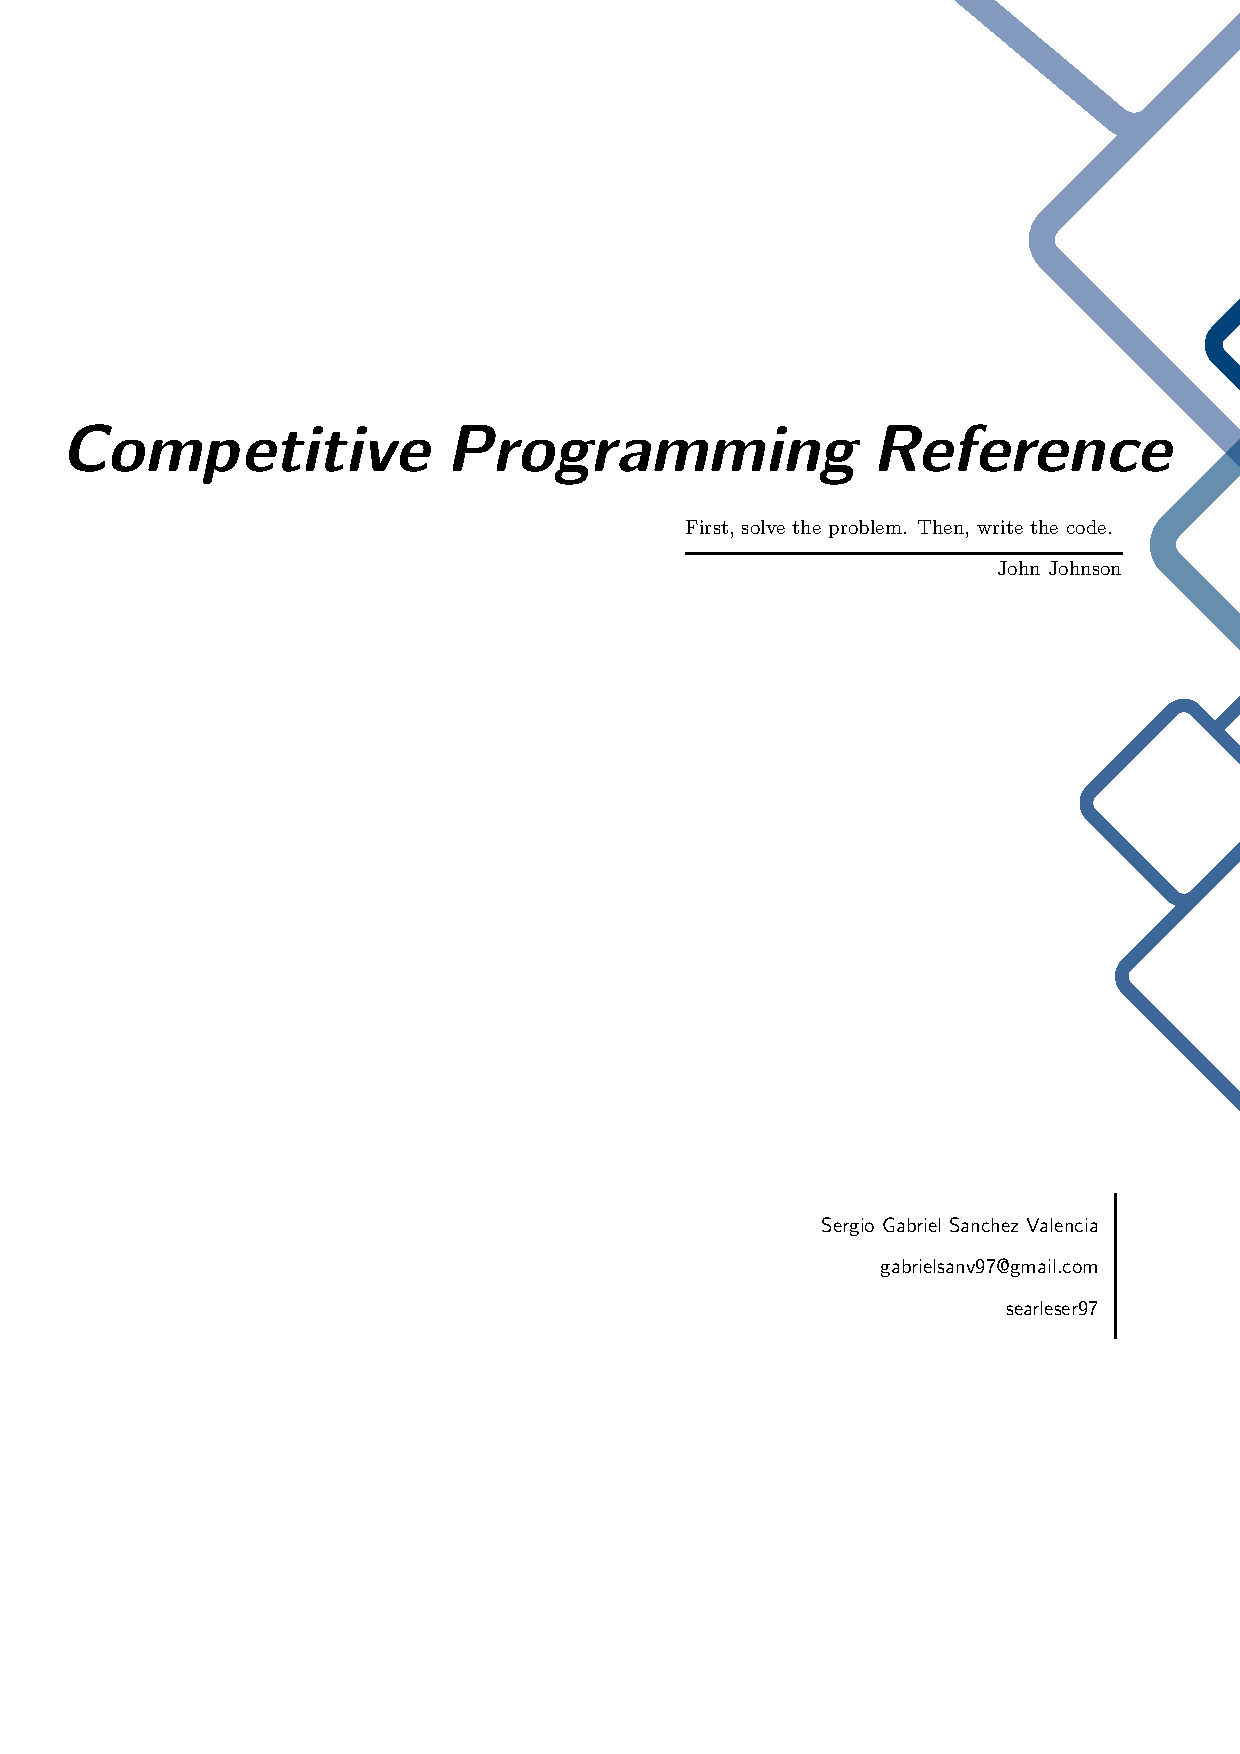
\includepdf{TitlePage.pdf}
\null
\thispagestyle{empty}
\newpage
\fontfamily{lmss}
\selectfont
\begin{multicols*}{2}
	\tableofcontents
	\newpage
	\cleardoublepage
\needspace{27\baselineskip}
\sectionfont{\bfseries\sffamily\centering\Huge}
\vspace{1em}
\section*{Coding Resources}
\markboth{CODING RESOURCES}{}
\addcontentsline{toc}{section}{Coding Resources}
\vspace{3em}
\subsectionfont{\bfseries\sffamily\centering\LARGE}
\vspace{0em}
\subsection*{C++}
\addcontentsline{toc}{subsection}{C++}
\vspace{2em}
\subsubsectionfont{\large\bfseries\sffamily\underline}
\subsubsection*{Competitive Programming Template}
\addcontentsline{toc}{subsubsection}{Competitive Programming Template}
\begin{minted}{cpp}
/****************************************************
https://searleser97.gitlab.io/algorithms/template.cpp
****************************************************/

#include <bits/stdc++.h>
using namespace std;
#define endl '\n'
#define forr(_, x, n) for (int _ = x; ~_; _--)
#define fos(_, x, n, s) for(int _ = x; _ < n; _ += s)
#define forn(_, x, n) fos (_, x, n, 1)
#define rep(_, n) forn(_, 0, n)
#define fi first
#define se second
#define pb push_back
#define pairii pair<int, int>
// typedef __int128_t lli;
typedef long long int li;
typedef long double ld;
\end{minted}
\vspace{-12pt}
\needspace{12\baselineskip}
\begin{minted}{cpp}
void _main(int tc) {

}

int main() {
  ios_base::sync_with_stdio(0);
  cin.tie(0), cout.tie(0);
  _main(0); return 0;
  int tc;
  cin >> tc;
  rep(i, tc) _main(i + 1);
}
\end{minted}

\needspace{6\baselineskip}
\subsubsectionfont{\large\bfseries\sffamily\underline}
\subsubsection*{Decimal Precision}
\addcontentsline{toc}{subsubsection}{Decimal Precision}
\begin{minted}{cpp}
// rounds up the decimal number
cout << setprecision(N) << n << endl;
// specify N fixed number of decimals
cout << fixed << setprecision(N) << n << endl;
\end{minted}

\needspace{4\baselineskip}
\subsubsectionfont{\large\bfseries\sffamily\underline}
\subsubsection*{Include All Libraries}
\addcontentsline{toc}{subsubsection}{Include All Libraries}
\begin{minted}{cpp}
#include <bits/stdc++.h>
using namespace std;
\end{minted}

\needspace{6\baselineskip}
\subsubsectionfont{\large\bfseries\sffamily\underline}
\subsubsection*{IO Optimization}
\addcontentsline{toc}{subsubsection}{IO Optimization}
\begin{minted}{cpp}
int main() {
  ios_base::sync_with_stdio(0);
  cin.tie(0);
}
\end{minted}

\needspace{7\baselineskip}
\subsubsectionfont{\large\bfseries\sffamily\underline}
\subsubsection*{Map Value To Int}
\addcontentsline{toc}{subsubsection}{Map Value To Int}
\begin{minted}{cpp}
// val = value
typedef string Val;
unordered_map<Val, int> intForVal;
unordered_map<int, Val> valForInt;
int mapId = 0;
\end{minted}
\vspace{-12pt}
\needspace{5\baselineskip}
\begin{minted}{cpp}
int Map(Val val) {
  if (intForVal.count(val)) return intForVal[val];
  valForInt[mapId] = val;
  return intForVal[val] = mapId++;
}

Val IMap(int n) { return valForInt[n]; }
\end{minted}
\vspace{-12pt}
\needspace{5\baselineskip}
\begin{minted}{cpp}
void initMapping() {
  mapId = 0;
  intForVal.clear();
  valForInt.clear();
}
\end{minted}

\needspace{12\baselineskip}
\subsubsectionfont{\large\bfseries\sffamily\underline}
\subsubsection*{Number To String}
\addcontentsline{toc}{subsubsection}{Number To String}
\begin{minted}{cpp}
#include <bits/stdc++.h>
using namespace std;

int main() {
  // to_string method converts any type of number
  // (int, double, long long int, ...) to string
  string str = "str+" + to_string(123 + 1);
  cout << str << endl;  // output: str+124
  return 0;
}
\end{minted}

\needspace{12\baselineskip}
\subsubsectionfont{\large\bfseries\sffamily\underline}
\subsubsection*{Permutations}
\addcontentsline{toc}{subsubsection}{Permutations}
\begin{minted}{cpp}
typedef vector<int> T;  // typedef string T;

vector<T> permutations(T v) {
  vector<vector<int>> ans;
  sort(v.begin(), v.end());
  do
    ans.push_back(v);
  while (next_permutation(v.begin(), v.end()));
  return ans;
}
\end{minted}

\needspace{11\baselineskip}
\subsubsectionfont{\large\bfseries\sffamily\underline}
\subsubsection*{Print Vector}
\addcontentsline{toc}{subsubsection}{Print Vector}
\begin{minted}{cpp}
void printv(vector<int> v) {
  if (v.size() == 0) {
    cout << "[]" << endl;
    return;
  }
  cout << "[" << v[0];
  for (int i = 1; i < v.size(); i++)
    cout << ", " << v[i];
  cout << "]" << endl;
}
\end{minted}

\needspace{6\baselineskip}
\subsubsectionfont{\large\bfseries\sffamily\underline}
\subsubsection*{Priority Queue Of Object}
\addcontentsline{toc}{subsubsection}{Priority Queue Of Object}
\begin{minted}{cpp}
struct Object {
  char first;
  int second;
};
\end{minted}
\vspace{-12pt}
\needspace{8\baselineskip}
\begin{minted}{cpp}
int main() {
  auto cmp = [](const Object& a, const Object& b) {
    return a.second > b.second;
  };
  priority_queue<Object, vector<Object>,
                 decltype(cmp)>
      pq(cmp);
}
\end{minted}

\needspace{10\baselineskip}
\subsubsectionfont{\large\bfseries\sffamily\underline}
\subsubsection*{Random}
\addcontentsline{toc}{subsubsection}{Random}
\begin{minted}{cpp}
mt19937_64 seed(chrono::steady_clock::now()
                    .time_since_epoch()
                    .count());

int random(int min, int max) {  // [min, max]
  return uniform_int_distribution<int>(min,
                                       max)(seed);
}
\end{minted}
\vspace{-12pt}
\needspace{4\baselineskip}
\begin{minted}{cpp}
double random(double min, double max) {  // [min, max)
  return uniform_real_distribution<double>(min,
                                           max)(seed);
}
\end{minted}

\needspace{10\baselineskip}
\subsubsectionfont{\large\bfseries\sffamily\underline}
\subsubsection*{Read Line}
\addcontentsline{toc}{subsubsection}{Read Line}
\begin{minted}{cpp}
// when reading lines, don't mix 'cin' with
// 'getline' just use getline and split
string input() {
  string ans;
  cin >> ws;
  cin.ignore(numeric_limits<streamsize>::max(), '\n');
  getline(cin, ans);
  return ans;
}
\end{minted}

\needspace{6\baselineskip}
\subsubsectionfont{\large\bfseries\sffamily\underline}
\subsubsection*{Set of Object}
\addcontentsline{toc}{subsubsection}{Set of Object}
\begin{minted}{cpp}
struct Object {
  char first;
  int second;
};
\end{minted}
\vspace{-12pt}
\needspace{6\baselineskip}
\begin{minted}{cpp}
int main() {
  auto cmp = [](const Object& a, const Object& b) {
    return a.second > b.second;
  };
  set<Object, decltype(cmp)> pq(cmp);
}
\end{minted}

\needspace{6\baselineskip}
\subsubsectionfont{\large\bfseries\sffamily\underline}
\subsubsection*{Sort Vector Of Object}
\addcontentsline{toc}{subsubsection}{Sort Vector Of Object}
\begin{minted}{cpp}
struct Object {
  char first;
  int second;
};
\end{minted}
\vspace{-12pt}
\needspace{3\baselineskip}
\begin{minted}{cpp}
bool cmp(const Object& a, const Object& b) {
  return a.second > b.second;
}
\end{minted}
\vspace{-12pt}
\needspace{6\baselineskip}
\begin{minted}{cpp}
int main() {
  vector<Object> v = {{'c', 3}, {'a', 1}, {'b', 2}};
  sort(v.begin(), v.end(), cmp);
}
\end{minted}

\needspace{5\baselineskip}
\subsubsectionfont{\large\bfseries\sffamily\underline}
\subsubsection*{Sort Vector of Pairs}
\addcontentsline{toc}{subsubsection}{Sort Vector of Pairs}
\begin{minted}{cpp}
vector<pair<int, int>> pairs;
// sorts array on the basis of the first element
sort(pairs.begin(), pairs.end());

\end{minted}

\needspace{10\baselineskip}
\subsubsectionfont{\large\bfseries\sffamily\underline}
\subsubsection*{Split String}
\addcontentsline{toc}{subsubsection}{Split String}
\begin{minted}{cpp}
vector<string> split(string str, char token) {
  stringstream ss(str);
  vector<string> v;
  while (getline(ss, str, token)) v.push_back(str);
  return v;
}
\end{minted}

\needspace{13\baselineskip}
\subsubsectionfont{\large\bfseries\sffamily\underline}
\subsubsection*{String To Int}
\addcontentsline{toc}{subsubsection}{String To Int}
\begin{minted}{cpp}
#include <bits/stdc++.h>
using namespace std;

int main() {
  int n = stoi("123") + 1;
  cout << n << endl;  // output: 124
  // stoll for long long int
  // stoull for unsigned long int
  // stod for double
  // stold for long double
}
\end{minted}

\needspace{5\baselineskip}
\subsubsectionfont{\large\bfseries\sffamily\underline}
\subsubsection*{Typedef}
\addcontentsline{toc}{subsubsection}{Typedef}
\begin{minted}{cpp}
typedef TYPE ALIAS;
// example:
typedef int T;
\end{minted}

\needspace{11\baselineskip}
\subsubsectionfont{\large\bfseries\sffamily\underline}
\subsubsection*{Unordered Map with pair as key}
\addcontentsline{toc}{subsubsection}{Unordered Map with pair as key}
\begin{minted}{cpp}
typedef int T;

struct pairhash {
  template <class T1, class T2>
  size_t operator()(const pair<T1, T2> &p) const {
    return hash<T1>{}(p.first) ^
           (hash<T2>{}(p.second) << 32);
  }
};
\end{minted}
\vspace{-12pt}
\needspace{5\baselineskip}
\begin{minted}{cpp}
int main() {
  unordered_map<pair<int, int>, T, hash_pair> um;
  um[{1, 2}] = 5;
  cout << um[{1, 2}] << endl;
}
\end{minted}

\needspace{8\baselineskip}
\subsectionfont{\bfseries\sffamily\centering\LARGE}
\vspace{0em}
\subsection*{Python}
\addcontentsline{toc}{subsection}{Python}
\vspace{2em}
\subsubsectionfont{\large\bfseries\sffamily\underline}
\subsubsection*{Combinations}
\addcontentsline{toc}{subsubsection}{Combinations}
\begin{minted}{py}
import itertools
# from arr choose k = > combinations(arr, k)
print(list(itertools.combinations([1, 2, 3], 3)))
\end{minted}

\needspace{17\baselineskip}
\subsubsectionfont{\large\bfseries\sffamily\underline}
\subsubsection*{Fast IO}
\addcontentsline{toc}{subsubsection}{Fast IO}
\begin{minted}{py}
from sys import stdin, stdout

N = 10
# Reads N chars from stdin(it counts '\n' as char)
stdin.read(N)
# Reads until '\n' or EOF
line = stdin.readline()
# Reads all lines in stdin until EOF
lines = stdin.readlines()
# Writes a string to stdout, it doesn't add '\n'
stdout.write(line)
# Writes a list of strings to stdout
stdout.writelines(lines)
# Reads numbers separated by space in a line
numbers = list(map(int, stdin.readline().split()))

\end{minted}

\needspace{4\baselineskip}
\subsubsectionfont{\large\bfseries\sffamily\underline}
\subsubsection*{Permutations}
\addcontentsline{toc}{subsubsection}{Permutations}
\begin{minted}{py}
import itertools
print(list(itertools.permutations([1, 2, 3])))

\end{minted}

\needspace{15\baselineskip}
\subsubsectionfont{\large\bfseries\sffamily\underline}
\subsubsection*{Random}
\addcontentsline{toc}{subsubsection}{Random}
\begin{minted}{py}
import random
# Initialize the random number generator.
random.seed(None)
# Returns a random integer N such that a <= N <= b.
random.randint(a, b)
# Returns a random integer N such that 0 <= N < b
random.randrange(b)
# Returns a random integer N such that a <= N < b.
random.randrange(a, b)
# Returns and integer with k random bits.
random.getrandbits(k)
# shuffles a list
random.shuffle(li)
\end{minted}

\needspace{7\baselineskip}
\subsubsectionfont{\large\bfseries\sffamily\underline}
\subsubsection*{Sort List}
\addcontentsline{toc}{subsubsection}{Sort List}
\begin{minted}{py}
li = ['a', 'c', 'b']
# sorts inplace in descending order
li.sort(reverse=True)
# returns sorted list ascending order
ol = sorted(li)
\end{minted}

\needspace{7\baselineskip}
\subsubsectionfont{\large\bfseries\sffamily\underline}
\subsubsection*{Sort List Of Object}
\addcontentsline{toc}{subsubsection}{Sort List Of Object}
\begin{minted}{py}
class MyObject :
  def __init__(self, first, second, third):
    self.first = first
    self.second = second
    self.third = third
\end{minted}
\vspace{-12pt}
\needspace{10\baselineskip}
\begin{minted}{py}
li = [MyObject('b', 3, 1), MyObject('a', 3, 2), MyObject('b', 3, 3)]
# returns list sorted by first then by second then by third in increasing order
ol = sorted(li, key = lambda x: (x.first, x.second, x.third), reverse=False)
# sorts inplace by first then by second then by third in increasing order
li.sort(key = lambda x: (x.first, x.second, x.third), reverse=False)

\end{minted}

\needspace{10\baselineskip}
\sectionfont{\bfseries\sffamily\centering\Huge}
\vspace{1em}
\section*{BITs Manipulation}
\markboth{BITS MANIPULATION}{}
\addcontentsline{toc}{section}{BITs Manipulation}
\vspace{3em}
\subsectionfont{\large\bfseries\sffamily\underline}
\subsection*{Bit Count}
\addcontentsline{toc}{subsection}{Bit Count}
\begin{minted}{cpp}
int bitCount(int n) {
  return sizeof(n) * 8 - __builtin_clz(n);
}
\end{minted}
\vspace{-12pt}
\needspace{5\baselineskip}
\begin{minted}{cpp}
int bitCount(int n) {
  int c = 0;
  while (n) c++, n >>= 1;
  return c;
}
\end{minted}

\needspace{13\baselineskip}
\subsectionfont{\large\bfseries\sffamily\underline}
\subsection*{Bits To Int}
\addcontentsline{toc}{subsection}{Bits To Int}
\begin{minted}{cpp}
typedef __int128_t lli

lli bitsToInt(string bits, bool isneg) {
  lli ans = 0;
  for (int i = bits.size() - 1, j = 0; ~i; i--, j++) {
    if (isneg) bits[i] = bits[i] == '0' ? '1' : '0';
    ans |= (lli)(bits[i] - '0') << j;
  }
  return isneg ? -(++ans) : ans;
}
\end{minted}

\needspace{8\baselineskip}
\subsectionfont{\large\bfseries\sffamily\underline}
\subsection*{Count Leading Zeroes}
\addcontentsline{toc}{subsection}{Count Leading Zeroes}
\begin{minted}{cpp}
int clz(int n) {
  return __builtin_clz(n);
  // return __builtin_clzl(n); for long
  // return __builtin_clzll(n); for long long
}
\end{minted}
\vspace{-12pt}
\needspace{6\baselineskip}
\begin{minted}{cpp}
int clz(int n) {
  // return sizeof(n) * 8 - bitCount(n);
  int c = 0;
  while (n) c++, n >>= 1;
  return sizeof(n) * 8 - c;
}
\end{minted}

\needspace{8\baselineskip}
\subsectionfont{\large\bfseries\sffamily\underline}
\subsection*{Count Set Bits}
\addcontentsline{toc}{subsection}{Count Set Bits}
\begin{minted}{cpp}
int popCount(int n) {
  return __builtin_popcount(n);
  // return __builtin_popcountl(n); for long
  // return __builtin_popcountll(n); for long long
}
\end{minted}
\vspace{-12pt}
\needspace{5\baselineskip}
\begin{minted}{cpp}
int popCount(int n) {
  int c = 0;
  while (n) c++, n &= n - 1;
  return c;
}
\end{minted}

\needspace{8\baselineskip}
\subsectionfont{\large\bfseries\sffamily\underline}
\subsection*{Count Trailing Zeroes}
\addcontentsline{toc}{subsection}{Count Trailing Zeroes}
\begin{minted}{cpp}
int ctz(int n) {
  return __builtin_ctz(n);
  // return __builtin_ctzl(n); for long
  // return __builtin_ctzll(n); for long long
}
\end{minted}
\vspace{-12pt}
\needspace{6\baselineskip}
\begin{minted}{cpp}
int ctz(int n) {
  int c = 0;
  n = ~n;
  while(n & 1) c++, n >>= 1;
  return c;
}
\end{minted}

\needspace{3\baselineskip}
\subsectionfont{\large\bfseries\sffamily\underline}
\subsection*{Divide By 2}
\addcontentsline{toc}{subsection}{Divide By 2}
\begin{minted}{cpp}
int divideBy2(int n) { return n >> 1; }
\end{minted}

\needspace{3\baselineskip}
\subsectionfont{\large\bfseries\sffamily\underline}
\subsection*{Is Even}
\addcontentsline{toc}{subsection}{Is Even}
\begin{minted}{cpp}
bool isEven(int n) { return ~n & 1; }
\end{minted}

\needspace{6\baselineskip}
\subsectionfont{\large\bfseries\sffamily\underline}
\subsection*{Is i-th Bit Set}
\addcontentsline{toc}{subsection}{Is i-th Bit Set}
\begin{minted}{cpp}
bool isIthBitSet(int n, int i) {
  return n & (1 << i);
}
\end{minted}

\needspace{3\baselineskip}
\subsectionfont{\large\bfseries\sffamily\underline}
\subsection*{Is Odd}
\addcontentsline{toc}{subsection}{Is Odd}
\begin{minted}{cpp}
bool isOdd(int n) { return n & 1; }
\end{minted}

\needspace{3\baselineskip}
\subsectionfont{\large\bfseries\sffamily\underline}
\subsection*{Is Power Of 2}
\addcontentsline{toc}{subsection}{Is Power Of 2}
\begin{minted}{cpp}
bool isPowerOf2(int n) { return n && !(n & (n - 1)); }
\end{minted}

\needspace{3\baselineskip}
\subsectionfont{\large\bfseries\sffamily\underline}
\subsection*{Least Significant Set Bit}
\addcontentsline{toc}{subsection}{Least Significant Set Bit}
\begin{minted}{cpp}
int lsb(int n) { return n & -n; }
\end{minted}

\needspace{6\baselineskip}
\subsectionfont{\large\bfseries\sffamily\underline}
\subsection*{Log2}
\addcontentsline{toc}{subsection}{Log2}
\begin{minted}{cpp}
int Log2(int n) {
  return sizeof(n) * 8 - __builtin_clz(n) - 1;
}
\end{minted}
\vspace{-12pt}
\needspace{5\baselineskip}
\begin{minted}{cpp}
int Log2(int n) {
  int lg2 = 0;
  while (n >>= 1) lg2++;
  return lg2;
}
\end{minted}

\needspace{6\baselineskip}
\subsectionfont{\large\bfseries\sffamily\underline}
\subsection*{Most Significant Set Bit}
\addcontentsline{toc}{subsection}{Most Significant Set Bit}
\begin{minted}{cpp}
int msb(int n) {
  return 1 << (sizeof(n) * 8 - __builtin_clz(n) - 1);
}
\end{minted}

\needspace{3\baselineskip}
\subsectionfont{\large\bfseries\sffamily\underline}
\subsection*{Multiply By 2}
\addcontentsline{toc}{subsection}{Multiply By 2}
\begin{minted}{cpp}
int multiplyBy2(int n) { return n << 1; }
\end{minted}

\needspace{3\baselineskip}
\subsectionfont{\large\bfseries\sffamily\underline}
\subsection*{One's Complement}
\addcontentsline{toc}{subsection}{One's Complement}
\begin{minted}{cpp}
int onesComplement(int n) { return ~n; }
\end{minted}

\needspace{8\baselineskip}
\subsectionfont{\large\bfseries\sffamily\underline}
\subsection*{Parity Check}
\addcontentsline{toc}{subsection}{Parity Check}
\begin{minted}{cpp}
bool parityCheck(int n) {
  return !__builtin_parity(n);
  // return !__builtin_parityl(n); for long
  // return !__builtin_parityll(n); for long long
}
\end{minted}
\vspace{-12pt}
\needspace{3\baselineskip}
\begin{minted}{cpp}
bool parityCheck(int n) {
  return isEven(popCount(n));
}
\end{minted}

\needspace{8\baselineskip}
\subsectionfont{\large\bfseries\sffamily\underline}
\subsection*{Print Bits}
\addcontentsline{toc}{subsection}{Print Bits}
\begin{minted}{cpp}
void printBits(int n) {
  for (int i = sizeof(n) * 8 - 1; ~i; i--)
    cout << ((n >> i) & 1);
  cout << endl;
}
\end{minted}

\needspace{3\baselineskip}
\subsectionfont{\large\bfseries\sffamily\underline}
\subsection*{Set i-th Bit}
\addcontentsline{toc}{subsection}{Set i-th Bit}
\begin{minted}{cpp}
int setIthBit(int n, int i) { return n | (1 << i); }
\end{minted}

\needspace{8\baselineskip}
\subsectionfont{\large\bfseries\sffamily\underline}
\subsection*{Swap Integer Variables}
\addcontentsline{toc}{subsection}{Swap Integer Variables}
\begin{minted}{cpp}
void swap(int &a, int &b) {
  a ^= b;
  b ^= a;
  a ^= b;
}
\end{minted}

\needspace{6\baselineskip}
\subsectionfont{\large\bfseries\sffamily\underline}
\subsection*{To Lower Case}
\addcontentsline{toc}{subsection}{To Lower Case}
\begin{minted}{cpp}
char lowerCase(char c) {
  return c | ' ';
}
\end{minted}

\needspace{6\baselineskip}
\subsectionfont{\large\bfseries\sffamily\underline}
\subsection*{To Upper Case}
\addcontentsline{toc}{subsection}{To Upper Case}
\begin{minted}{cpp}
char upperCase(char c) {
  return c & '_';
}
\end{minted}

\needspace{6\baselineskip}
\subsectionfont{\large\bfseries\sffamily\underline}
\subsection*{Toggle Case}
\addcontentsline{toc}{subsection}{Toggle Case}
\begin{minted}{cpp}
char toggleCase(char c) {
  return c ^ ' ';
}
\end{minted}

\needspace{6\baselineskip}
\subsectionfont{\large\bfseries\sffamily\underline}
\subsection*{Toggle i-th Bit}
\addcontentsline{toc}{subsection}{Toggle i-th Bit}
\begin{minted}{cpp}
int toggleIthBit(int n, int i) {
  return n ^ (1 << i);
}
\end{minted}

\needspace{3\baselineskip}
\subsectionfont{\large\bfseries\sffamily\underline}
\subsection*{Two's Complement}
\addcontentsline{toc}{subsection}{Two's Complement}
\begin{minted}{cpp}
int twosComplement(int n) { return ~n + 1; }
\end{minted}

\needspace{6\baselineskip}
\subsectionfont{\large\bfseries\sffamily\underline}
\subsection*{Unset i-th Bit}
\addcontentsline{toc}{subsection}{Unset i-th Bit}
\begin{minted}{cpp}
int unsetIthBit(int n, int i) {
  return n & (~(1 << i));
}
\end{minted}

\needspace{17\baselineskip}
\sectionfont{\bfseries\sffamily\centering\Huge}
\vspace{1em}
\section*{Data Structures}
\markboth{DATA STRUCTURES}{}
\addcontentsline{toc}{section}{Data Structures}
\vspace{3em}
\subsectionfont{\bfseries\sffamily\centering\LARGE}
\vspace{0em}
\subsection*{Geometry}
\addcontentsline{toc}{subsection}{Geometry}
\vspace{2em}
\subsubsectionfont{\large\bfseries\sffamily\underline}
\subsubsection*{Circle}
\addcontentsline{toc}{subsubsection}{Circle}
\begin{minted}{cpp}
// c = center, r = radius;
#include "Point.cpp"

struct Circle {
  Point c;
  ld r;
  Circle(Point c, ld r) : c(c), r(r) {}
};
\end{minted}

\needspace{9\baselineskip}
\subsubsectionfont{\large\bfseries\sffamily\underline}
\subsubsection*{Point}
\addcontentsline{toc}{subsubsection}{Point}
\begin{minted}{cpp}
typedef long double ld;
const ld pi = acos(-1);

struct Point {
  ld x, y;
  Point() : x(0), y(0) {}
  Point(ld x, ld y) : x(x), y(y) {}
\end{minted}
\vspace{-12pt}
\needspace{3\baselineskip}
\begin{minted}{cpp}
  Point operator+(const Point &p) {
    return Point(x + p.x, y + p.y);
  }
\end{minted}
\vspace{-12pt}
\needspace{3\baselineskip}
\begin{minted}{cpp}
  Point operator-(const Point &p) {
    return Point(x - p.x, y - p.y);
  }
\end{minted}
\vspace{-12pt}
\needspace{3\baselineskip}
\begin{minted}{cpp}
  Point operator*(const ld &k) {
    return Point(x * k, y * k);
  }
\end{minted}
\vspace{-12pt}
\needspace{3\baselineskip}
\begin{minted}{cpp}
  Point operator/(const ld &k) {
    return Point(x / k, y / k);
  }
\end{minted}
\vspace{-12pt}
\needspace{3\baselineskip}
\begin{minted}{cpp}
  ld dot(const Point &p) {
    return x * p.x + y * p.y;
  }
\end{minted}
\vspace{-12pt}
\needspace{3\baselineskip}
\begin{minted}{cpp}
  ld cross(const Point &p) {
    return x * p.y - y * p.x;
  }
\end{minted}
\vspace{-12pt}
\needspace{3\baselineskip}
\begin{minted}{cpp}
  ld norm() const { return sqrt(x * x + y * y); }
  Point perpendicularLeft() { return Point(-y, x); }
  Point perpendicularRight() { return Point(y, -x); }
\end{minted}
\vspace{-12pt}
\needspace{6\baselineskip}
\begin{minted}{cpp}
  Point rotate(ld deg) {
    ld rad = (deg * pi) / 180.0;
    return Point(x * cos(rad) - y * sin(rad),
                 x * sin(rad) + y * cos(rad));
  }
};
\end{minted}

\needspace{12\baselineskip}
\subsectionfont{\bfseries\sffamily\centering\LARGE}
\vspace{0em}
\subsection*{Graphs}
\addcontentsline{toc}{subsection}{Graphs}
\vspace{2em}
\subsubsectionfont{\large\bfseries\sffamily\underline}
\subsubsection*{Union Find}
\addcontentsline{toc}{subsubsection}{Union Find}
\begin{minted}{cpp}
struct UnionFind {
  int n;
  vector<int> dad, size;

  UnionFind(int N) : n(N), dad(N), size(N, 1) {
    while (N--) dad[N] = N;
  }
\end{minted}
\vspace{-12pt}
\needspace{4\baselineskip}
\begin{minted}{cpp}
  // O(lg*(N))
  int root(int u) {
    if (dad[u] == u) return u;
    return dad[u] = root(dad[u]);
  }
\end{minted}
\vspace{-12pt}
\needspace{8\baselineskip}
\begin{minted}{cpp}
  // O(1)
  void join(int u, int v) {
    int Ru = root(u), Rv = root(v);
    if (Ru == Rv) return;
    if (size[Ru] > size[Rv]) swap(Ru, Rv);
    --n, dad[Ru] = Rv;
    size[Rv] += size[Ru];
  }
\end{minted}
\vspace{-12pt}
\needspace{4\baselineskip}
\begin{minted}{cpp}
  // O(lg*(N))
  bool areConnected(int u, int v) {
    return root(u) == root(v);
  }
\end{minted}
\vspace{-12pt}
\needspace{4\baselineskip}
\begin{minted}{cpp}
  int getSize(int u) { return size[root(u)]; }

  int numberOfSets() { return n; }
};
\end{minted}

\needspace{11\baselineskip}
\subsubsectionfont{\large\bfseries\sffamily\underline}
\subsubsection*{Union Find (Partially Persistent)}
\addcontentsline{toc}{subsubsection}{Union Find (Partially Persistent)}
\begin{minted}{cpp}
// jTime = join time, t = time
struct UnionFind {
  int Time = 0;
  vector<int> dad, size, jTime;

  UnionFind(int N) : dad(N), size(N, 1), jTime(N) {
    while (N--) dad[N] = N;
  }
\end{minted}
\vspace{-12pt}
\needspace{5\baselineskip}
\begin{minted}{cpp}
  // O(lg(N))
  int root(int u, int t) {
    while (jTime[u] <= t && u != dad[u]) u = dad[u];
    return u;
  }
\end{minted}
\vspace{-12pt}
\needspace{10\baselineskip}
\begin{minted}{cpp}
  // O(1)
  void join(int u, int v, bool newTime = 1) {
    int Ru = root(u, Time), Rv = root(v, Time);
    if (newTime) Time++;
    if (Ru == Rv) return;
    if (size[Ru] > size[Rv]) swap(Ru, Rv);
    jTime[Ru] = Time;
    dad[Ru] = Rv;
    size[Rv] += size[Ru];
  }
\end{minted}
\vspace{-12pt}
\needspace{4\baselineskip}
\begin{minted}{cpp}
  // O(lg(N))
  bool areConnected(int u, int v, int t) {
    return root(u, t) == root(v, t);
  }
\end{minted}
\vspace{-12pt}
\needspace{4\baselineskip}
\begin{minted}{cpp}
  // O(lg(N))
  int getLastVersionSize(int u) {
    return size[root(u, Time)];
  }
\end{minted}
\vspace{-12pt}
\needspace{13\baselineskip}
\begin{minted}{cpp}
  // O(lg(Time) * lg(N))
  int joinTime(int u, int v) {
    int l = 0, r = Time, ans = -1;
    while (l <= r) {
      int mid = (l + r) >> 1;
      if (areConnected(u, v, mid))
        ans = mid, r = mid - 1;
      else
        l = mid + 1;
    }
    return ans;
  }
};
\end{minted}

\needspace{8\baselineskip}
\subsectionfont{\bfseries\sffamily\centering\LARGE}
\vspace{0em}
\subsection*{Ranges}
\addcontentsline{toc}{subsection}{Ranges}
\vspace{2em}
\subsubsectionfont{\large\bfseries\sffamily\underline}
\subsubsection*{BIT}
\addcontentsline{toc}{subsubsection}{BIT}
\begin{minted}{cpp}
template <class T>
struct BIT {
  T neutro = 0;
  vector<T> bit;
\end{minted}
\vspace{-12pt}
\needspace{7\baselineskip}
\begin{minted}{cpp}
  BIT(int n) { bit.assign(++n, neutro); }

  inline T F(T a, T b) {
    return a + b;
    // return a * b;
  }
\end{minted}
\vspace{-12pt}
\needspace{5\baselineskip}
\begin{minted}{cpp}
  // Inverse of F
  inline T I(T a, T b) {
    return a - b;
    // return a / b;
  }
\end{minted}
\vspace{-12pt}
\needspace{7\baselineskip}
\begin{minted}{cpp}
  // O(N)
  void build() {
    for (int i = 1; i < bit.size(); i++) {
      int j = i + (i & -i);
      if (j < bit.size()) bit[j] = F(bit[j], bit[i]);
    }
  }
\end{minted}
\vspace{-12pt}
\needspace{4\baselineskip}
\begin{minted}{cpp}
  // O(lg(N))
  void update(int i, T val) {
    for (i++; i < bit.size(); i += i & -i)
      bit[i] = F(bit[i], val);
  }
\end{minted}
\vspace{-12pt}
\needspace{6\baselineskip}
\begin{minted}{cpp}
  // O(lg(N))
  T query(int i) {
    T ans = neutro;
    for (i++; i; i -= i & -i) ans = F(ans, bit[i]);
    return ans;
  }
\end{minted}
\vspace{-12pt}
\needspace{6\baselineskip}
\begin{minted}{cpp}
  // O(lg(N)), [l, r]
  T query(int l, int r) {
    return I(query(r), query(--l));
  }

  T& operator[](int i) { return bit[++i]; }
};
\end{minted}

\needspace{5\baselineskip}
\subsubsectionfont{\large\bfseries\sffamily\underline}
\subsubsection*{BIT Range Update}
\addcontentsline{toc}{subsubsection}{BIT Range Update}
\begin{minted}{cpp}
typedef long long int T;
T neutro = 0;
vector<T> bit1, bit2;
\end{minted}
\vspace{-12pt}
\needspace{4\baselineskip}
\begin{minted}{cpp}
void initVars(int n) {
  bit1.assign(++n, neutro);
  bit2 = bit1;
}
\end{minted}
\vspace{-12pt}
\needspace{5\baselineskip}
\begin{minted}{cpp}
// O(lg(N))
void update(vector<T> &bit, int i, T val) {
  for (i++; i < bit.size(); i += i & -i)
    bit[i] += val;
}
\end{minted}
\vspace{-12pt}
\needspace{7\baselineskip}
\begin{minted}{cpp}
// O(lg(N)), [l, r]
void update(int l, int r, T val) {
  update(bit1, l, val);
  update(bit1, r + 1, -val);
  update(bit2, r + 1, val * r);
  update(bit2, l, -val * (l - 1));
}
\end{minted}
\vspace{-12pt}
\needspace{6\baselineskip}
\begin{minted}{cpp}
// O(lg(N))
T query(vector<T> &bit, int i) {
  T ans = neutro;
  for (i++; i; i -= i & -i) ans += bit[i];
  return ans;
}
\end{minted}
\vspace{-12pt}
\needspace{4\baselineskip}
\begin{minted}{cpp}
// O(lg(N))
T query(int i) {
  return query(bit1, i) * i + query(bit2, i);
}
\end{minted}
\vspace{-12pt}
\needspace{4\baselineskip}
\begin{minted}{cpp}
// O(lg(N)), [l, r]
T query(int l, int r) {
  return query(r) - query(l - 1);
}
\end{minted}

\needspace{6\baselineskip}
\subsubsectionfont{\large\bfseries\sffamily\underline}
\subsubsection*{Segment Tree}
\addcontentsline{toc}{subsubsection}{Segment Tree}
\begin{minted}{cpp}
// st = segment tree. st[1] = root;
// neutro = operation neutral value
// e.g. for sum is 0, for multiplication
// is 1, for gcd is 0, for min is INF, etc.
\end{minted}
\vspace{-12pt}
\needspace{5\baselineskip}
\begin{minted}{cpp}
template <class T>
struct SegmentTree {
  T neutro = 0;
  int N;
  vector<T> st;
\end{minted}
\vspace{-12pt}
\needspace{8\baselineskip}
\begin{minted}{cpp}
  SegmentTree(int n) : st(2 * n, neutro), N(n) {}

  inline T F(T a, T b) {
    return a + b;
    // return __gcd(a, b);
    // return a * b;
    // return min(a, b);
  }
\end{minted}
\vspace{-12pt}
\needspace{5\baselineskip}
\begin{minted}{cpp}
  // O(2N)
  void build() {
    for (int i = N - 1; i > 0; i--)
      st[i] = F(st[i << 1], st[i << 1 | 1]);
  }
\end{minted}
\vspace{-12pt}
\needspace{5\baselineskip}
\begin{minted}{cpp}
  // O(lg(2N)), works like replacing arr[i] with val
  void update(int i, T val) {
    for (st[i += N] = val; i > 1; i >>= 1)
      st[i >> 1] = F(st[i], st[i ^ 1]);
  }
\end{minted}
\vspace{-12pt}
\needspace{9\baselineskip}
\begin{minted}{cpp}
  // O(3N), [l, r]
  void update(int l, int r, T val) {
    if (l == r)
      update(l, val);
    else {
      for (l += N, r += N; l <= r; l++) st[l] = val;
      build();
    }
  }
\end{minted}
\vspace{-12pt}
\needspace{9\baselineskip}
\begin{minted}{cpp}
  // O(lg(2N)), [l, r]
  T query(int l, int r) {
    T ans = neutro;
    for (l += N, r += N; l <= r; l >>= 1, r >>= 1) {
      if (l & 1) ans = F(ans, st[l++]);
      if (~r & 1) ans = F(ans, st[r--]);
    }
    return ans;
  }
\end{minted}
\vspace{-12pt}
\needspace{2\baselineskip}
\begin{minted}{cpp}
  T& operator[](int i) { return st[i + N]; }
};
\end{minted}

\needspace{7\baselineskip}
\subsubsectionfont{\large\bfseries\sffamily\underline}
\subsubsection*{Segment Tree Lazy Propagation}
\addcontentsline{toc}{subsubsection}{Segment Tree Lazy Propagation}
\begin{minted}{cpp}
// st = segment tree, st[1] = root, H = height of d
// u = updates, d = delayed updates
// neutro = operation neutral val
// e.g. for sum is 0, for multiplication
// is 1, for gcd is 0, for min is INF, etc.
\end{minted}
\vspace{-12pt}
\needspace{6\baselineskip}
\begin{minted}{cpp}
template <class T>
struct SegmentTree {
  T neutro = 0;
  int N, H;
  vector<T> st, d;
  vector<bool> u;
\end{minted}
\vspace{-12pt}
\needspace{4\baselineskip}
\begin{minted}{cpp}
  SegmentTree(int n, T val)
      : st(2 * n, val), d(n), u(n) {
    H = sizeof(int) * 8 - __builtin_clz(N = n);
  }
\end{minted}
\vspace{-12pt}
\needspace{4\baselineskip}
\begin{minted}{cpp}
  inline T kTimesF(T a, T k) {
    return a * k;
    // return pow(a, k);
    // return a;
  }
  \end{minted}
\vspace{-12pt}
\needspace{6\baselineskip}
\begin{minted}{cpp}
  inline T F(T a, T b) {
    return a + b;
    // return a * b;
    // return __gcd(a, b);
    // return min(a, b);
  }
\end{minted}
\vspace{-12pt}
\needspace{4\baselineskip}
\begin{minted}{cpp}
  inline T UF(T a, T b) {
    return b;  // replace update
    // return F(a, b); // apply F to current value
  }
\end{minted}
\vspace{-12pt}
\needspace{4\baselineskip}
\begin{minted}{cpp}
  void apply(int i, T val, int k) {
    st[i] = UF(st[i], kTimesF(val, k));
    if (i < N) d[i] = UF(d[i], val), u[i] = 1;
  }
\end{minted}
\vspace{-12pt}
\needspace{3\baselineskip}
\begin{minted}{cpp}
  void calc(int i) {
    if (!u[i]) st[i] = F(st[i << 1], st[i << 1 | 1]);
  }
\end{minted}
\vspace{-12pt}
\needspace{4\baselineskip}
\begin{minted}{cpp}
  // O(2N)
  void build() {
    for (int i = N - 1; i > 0; i--) calc(i);
  }
\end{minted}
\vspace{-12pt}
\needspace{4\baselineskip}
\begin{minted}{cpp}
  // O(lg(N))
  void build(int p) {
    while (p > 1) p >>= 1, calc(p);
  }
\end{minted}
\vspace{-12pt}
\needspace{12\baselineskip}
\begin{minted}{cpp}
  // O(lg(N))
  void push(int p) {
    for (int s = H, k = 1 << (H - 1); s > 0;
         s--, k >>= 1) {
      int i = p >> s;
      if (u[i]) {
        apply(i << 1, d[i], k);
        apply(i << 1 | 1, d[i], k);
        u[i] = 0, d[i] = neutro;
      }
    }
  }
\end{minted}
\vspace{-12pt}
\needspace{12\baselineskip}
\begin{minted}{cpp}
  // O(lg(N)), [l, r]
  void update(int l, int r, T val) {
    push(l += N);
    push(r += N);
    int ll = l, rr = r, k = 1;
    for (; l <= r; l >>= 1, r >>= 1, k <<= 1) {
      if (l & 1) apply(l++, val, k);
      if (~r & 1) apply(r--, val, k);
    }
    build(ll);
    build(rr);
  }
\end{minted}
\vspace{-12pt}
\needspace{11\baselineskip}
\begin{minted}{cpp}
  // O(lg(2N)), [l, r]
  T query(int l, int r) {
    push(l += N);
    push(r += N);
    T ans = neutro;
    for (; l <= r; l >>= 1, r >>= 1) {
      if (l & 1) ans = F(ans, st[l++]);
      if (~r & 1) ans = F(ans, st[r--]);
    }
    return ans;
  }
\end{minted}
\vspace{-12pt}
\needspace{2\baselineskip}
\begin{minted}{cpp}
  T& operator[](int i) { return st[i + N]; }
};
\end{minted}

\needspace{6\baselineskip}
\subsubsectionfont{\large\bfseries\sffamily\underline}
\subsubsection*{Sparse Table}
\addcontentsline{toc}{subsubsection}{Sparse Table}
\begin{minted}{cpp}
// st = sparse table, Arith = Arithmetic
typedef int T;
int neutro = 0;
vector<vector<T>> st;
\end{minted}
\vspace{-12pt}
\needspace{6\baselineskip}
\begin{minted}{cpp}
T F(T a, T b) {
  // return min(a, b);
  return __gcd(a, b);
  // return a + b; // Arith
  // return a * b; // Arith
}
\end{minted}
\vspace{-12pt}
\needspace{9\baselineskip}
\begin{minted}{cpp}
// O(Nlg(N))
void build(vector<T> &arr) {
  st.assign(log2(arr.size()), vector<T>(arr.size()));
  st[0] = arr;
  for (int i = 1; (1 << i) <= arr.size(); i++)
    for (int j = 0; j + (1 << i) <= arr.size(); j++)
      st[i][j] = F(st[i - 1][j],
                   st[i - 1][j + (1 << (i - 1))]);
}
\end{minted}
\vspace{-12pt}
\needspace{5\baselineskip}
\begin{minted}{cpp}
// O(1), [l, r]
T query(int l, int r) {
  int i = log2(r - l + 1);
  return F(st[i][l], st[i][r + 1 - (1 << i)]);
}
\end{minted}
\vspace{-12pt}
\needspace{11\baselineskip}
\begin{minted}{cpp}
// O(lg(N)), [l, r]
T queryArith(int l, int r) {
  T ans = neutro;
  while (true) {
    int k = log2(r - l + 1);
    ans = F(ans, st[k][l]);
    l += 1 << k;
    if (l > r) break;
  }
  return ans;
}
\end{minted}

\needspace{10\baselineskip}
\subsubsectionfont{\large\bfseries\sffamily\underline}
\subsubsection*{Wavelet Tree}
\addcontentsline{toc}{subsubsection}{Wavelet Tree}
\begin{minted}{cpp}
// pref = prefix sum
// lte = less than or equal, 1-indexed
// A = max_element(from, to)
// lcount = left children count
struct WaveletTree {
  WaveletTree *l, *r;
  int lo, hi;
  vector<int> lcount, pref;
\end{minted}
\vspace{-12pt}
\needspace{17\baselineskip}
\begin{minted}{cpp}
  // O(N*lg(A))
  WaveletTree(vector<int>::iterator from,
              vector<int>::iterator to, int lo,
              int hi) {
    this->lo = lo, this->hi = hi;
    if (lo == hi or from >= to) return;
    int mid = (lo + hi) >> 1;
    auto f = [mid](int x) { return x <= mid; };
    lcount.reserve(to - from + 1);
    pref.reserve(to - from + 1);
    lcount.push_back(0);
    pref.push_back(0);
    for (auto it = from; it != to; it++)
      lcount.push_back(lcount.back() + f(*it)),
          pref.push_back(pref.back() + *it);
    auto pivot = stable_partition(from, to, f);
    l = new WaveletTree(from, pivot, lo, mid);
    r = new WaveletTree(pivot, to, mid + 1, hi);
  }
\end{minted}
\vspace{-12pt}
\needspace{9\baselineskip}
\begin{minted}{cpp}
  // O(lg(A)) frequency of k in [a, b]
  int freq(int a, int b, int k) {
    if (a > b or k < lo or k > hi) return 0;
    if (lo == hi) return b - a + 1;
    int lc = lcount[a - 1], rc = lcount[b];
    if (k > ((lo + hi) >> 1))
      return r->freq(a - lc, b - rc, k);
    return l->freq(lc + 1, rc, k);
  }
\end{minted}
\vspace{-12pt}
\needspace{10\baselineskip}
\begin{minted}{cpp}
  // O(lg(A)) kth-Smallest element in [a, b]
  int kth(int a, int b, int k) {
    if (a > b) return 0;
    if (lo == hi) return lo;
    int lc = lcount[a - 1], rc = lcount[b],
        inleft = rc - lc;
    if (k > inleft)
      return r->kth(a - lc, b - rc, k - inleft);
    return l->kth(lc + 1, rc, k);
  }
\end{minted}
\vspace{-12pt}
\needspace{8\baselineskip}
\begin{minted}{cpp}
  // O(lg(A)) count of elements <= to k in [a, b]
  int lte(int a, int b, int k) {
    if (a > b or k < lo) return 0;
    if (hi <= k) return b - a + 1;
    int lc = lcount[a - 1], rc = lcount[b];
    return l->lte(lc + 1, rc, k) +
           r->lte(a - lc, b - rc, k);
  }
\end{minted}
\vspace{-12pt}
\needspace{8\baselineskip}
\begin{minted}{cpp}
  // O(lg(A)) sum of numbers <= to k in [a, b]
  int sumlte(int a, int b, int k) {
    if (a > b or k < lo) return 0;
    if (hi <= k) return pref[b] - pref[a - 1];
    int lc = lcount[a - 1], rc = lcount[b];
    return l->sumlte(lc + 1, rc, k) +
           r->sumlte(a - lc, b - rc, k);
  }
};
\end{minted}

\needspace{13\baselineskip}
\subsubsectionfont{\large\bfseries\sffamily\underline}
\subsubsection*{Wavelet Tree Compressed}
\addcontentsline{toc}{subsubsection}{Wavelet Tree Compressed}
\begin{minted}{cpp}
// lte = less than or equal, c = compressed
// o  = original, 0-indexed
#include "../../Techniques/Binary Search.cpp"
#include "Wavelet Tree.cpp"

template <class T>
struct WaveletTreeCompressed {
  unordered_map<int, T> imap;
  unordered_map<T, int> Map;
  WaveletTree* wt;
  vector<T> o;
\end{minted}
\vspace{-12pt}
\needspace{12\baselineskip}
\begin{minted}{cpp}
  // O(N*lg(N))
  WaveletTreeCompressed(vector<T>& v) {
    o = v;
    int inf = 1 << 30, n = 0, lo = inf, hi = -inf;
    set<T> s(v.begin(), v.end());
    vector<int> c(v.size());
    for (auto& e : s) Map[e] = n++;
    for (int i = 0; i < v.size(); i++)
      c[i] = Map[v[i]], imap[Map[v[i]]] = v[i];
    for (auto& e : c)
      lo = min(lo, e), hi = max(hi, e);
    wt = new WaveletTree(c.begin(), c.end(), lo, hi);
  }
\end{minted}
\vspace{-12pt}
\needspace{4\baselineskip}
\begin{minted}{cpp}
  // O(lg(N)) frequency of k in [a, b]
  int freq(int l, int r, T k) {
    return wt->freq(++l, ++r, Map[k]);
  }
\end{minted}
\vspace{-12pt}
\needspace{4\baselineskip}
\begin{minted}{cpp}
  // O(lg(N)) kth-Smallest element in [l, r]
  T kth(int l, int r, int k) {
    return imap[wt->kth(++l, ++r, k)];
  }
\end{minted}
\vspace{-12pt}
\needspace{5\baselineskip}
\begin{minted}{cpp}
  // O(lg(N)) count of numbers <= to k in [l, r]
  T lte(int l, int r, T k) {
    int kk = Map[bSearch<T>(o, k, l, r)[1]];
    return imap[wt->lte(++l, ++r, kk)];
  }
\end{minted}
\vspace{-12pt}
\needspace{5\baselineskip}
\begin{minted}{cpp}
  // O(lg(N)) sum of numbers <= to k in [l, r]
  T sumlte(int l, int r, T k) {
    int kk = Map[bSearch<T>(o, k, l, r)[1]];
    return imap[wt->sumlte(++l, ++r, kk)];
  }
};
\end{minted}

\needspace{9\baselineskip}
\subsectionfont{\bfseries\sffamily\centering\LARGE}
\vspace{0em}
\subsection*{Strings}
\addcontentsline{toc}{subsection}{Strings}
\vspace{2em}
\subsubsectionfont{\large\bfseries\sffamily\underline}
\subsubsection*{Suffix Automaton}
\addcontentsline{toc}{subsubsection}{Suffix Automaton}
\begin{minted}{cpp}
// link[u]: links to the longest suffix which is
//          not in the same endpos-equivalence class
// len[u]: length of the longest suffix that
//         corresponds to u's endpos-equivalence class
\end{minted}
\vspace{-12pt}
\needspace{4\baselineskip}
\begin{minted}{cpp}
struct SuffixAutomaton {
  vector<int> len, link, isClone, first;
  vector<map<char, int>> next;
  int size, last;
\end{minted}
\vspace{-12pt}
\needspace{5\baselineskip}
\begin{minted}{cpp}
  void init(int n) {
    first = isClone = len = link = vector<int>(2 * n);
    next.resize(2 * n);
    len[0] = 0, link[0] = -1, size = 1, last = 0;
  }
\end{minted}
\vspace{-12pt}
\needspace{5\baselineskip}
\begin{minted}{cpp}
  // O(N)
  SuffixAutomaton(const string& s) {
    init(s.size());
    for (const auto& c : s) add(c);
  }
\end{minted}
\vspace{-12pt}
\needspace{22\baselineskip}
\begin{minted}{cpp}
  // O(1)
  void add(const char& c) {
    int p = last, u = size++;
    len[u] = len[p] + 1, first[u] = len[p];
    while (p != -1 && !next[p].count(c))
      next[p][c] = u, p = link[p];
    if (p == -1) link[u] = 0;
    else {
      int q = next[p][c];
      if (len[p] + 1 == len[q]) link[u] = q;
      else {
        int clone = size++;
        first[clone] = first[q];
        len[clone] = len[p] + 1, isClone[clone] = 1;
        link[clone] = link[q], next[clone] = next[q];
        while (p != -1 && next[p][c] == q)
          next[p][c] = clone, p = link[p];
        link[q] = link[u] = clone;
      }
    }
    last = u;
  }
\end{minted}
\vspace{-12pt}
\needspace{7\baselineskip}
\begin{minted}{cpp}
  // O(N)
  unordered_set<int> getTerminals() {
    unordered_set<int> terminals;
    for (int p = last; p; p = link[p])
      terminals.insert(p);
    return terminals;
  }
};
\end{minted}

\needspace{5\baselineskip}
\subsubsectionfont{\large\bfseries\sffamily\underline}
\subsubsection*{Trie}
\addcontentsline{toc}{subsubsection}{Trie}
\begin{minted}{cpp}
// wpt = number of words passing through
// w = number of words ending in the node
// c = character
\end{minted}
\vspace{-12pt}
\needspace{8\baselineskip}
\begin{minted}{cpp}
struct Trie {

  struct Node {
    // for lexicographical order use 'map'
    // map<char, Node *> ch;
    unordered_map<char, Node *> ch;
    int w = 0, wpt = 0;
  };
\end{minted}
\vspace{-12pt}
\needspace{12\baselineskip}
\begin{minted}{cpp}
  Node *root = new Node();

  // O(STR.SIZE)
  void insert(string str) {
    Node *curr = root;
    for (auto &c : str) {
      if (!curr->ch.count(c))
        curr->ch[c] = new Node();
      curr->wpt++, curr = curr->ch[c];
    }
    curr->wpt++, curr->w++;
  }
\end{minted}
\vspace{-12pt}
\needspace{9\baselineskip}
\begin{minted}{cpp}
  // O(STR.SIZE)
  Node *find(string &str) {
    Node *curr = root;
    for (auto &c : str) {
      if (!curr->ch.count(c)) return nullptr;
      curr = curr->ch[c];
    }
    return curr;
  }
\end{minted}
\vspace{-12pt}
\needspace{5\baselineskip}
\begin{minted}{cpp}
  // O(STR.SIZE) number of words with given prefix
  int prefixCount(string prefix) {
    Node *node = find(prefix);
    return node ? node->wpt : 0;
  }
\end{minted}
\vspace{-12pt}
\needspace{5\baselineskip}
\begin{minted}{cpp}
  // O(STR.SIZE) number of words matching str
  int strCount(string str) {
    Node *node = find(str);
    return node ? node->w : 0;
  }
\end{minted}
\vspace{-12pt}
\needspace{10\baselineskip}
\begin{minted}{cpp}
  // O(N)
  void getWords(Node *curr, vector<string> &words,
                string &word) {
    if (!curr) return;
    if (curr->w) words.push_back(word);
    for (auto &c : curr->ch) {
      getWords(c.second, words, word += c.first);
      word.pop_back();
    }
  }
\end{minted}
\vspace{-12pt}
\needspace{7\baselineskip}
\begin{minted}{cpp}
  // O(N)
  vector<string> getWords() {
    vector<string> words;
    string word = "";
    getWords(root, words, word);
    return words;
  }
\end{minted}
\vspace{-12pt}
\needspace{5\baselineskip}
\begin{minted}{cpp}
  // O(N)
  vector<string> getWordsByPrefix(string prefix) {
    vector<string> words;
    getWords(find(prefix), words, prefix);
  }
\end{minted}
\vspace{-12pt}
\needspace{15\baselineskip}
\begin{minted}{cpp}
  // O(STR.SIZE)
  bool remove(Node *curr, string &str, int &i) {
    if (i == str.size()) {
      curr->wpt--;
      return curr->w ? !(curr->w = 0) : 0;
    }
    int c = str[i];
    if (!curr->ch.count(c)) return false;
    if (remove(curr->ch[c], str, ++i)) {
      if (!curr->ch[c]->wpt)
        curr->wpt--, curr->ch.erase(c);
      return true;
    }
    return false;
  }
\end{minted}
\vspace{-12pt}
\needspace{6\baselineskip}
\begin{minted}{cpp}
  // O(STR.SIZE)
  int remove(string str) {
    int i = 0;
    return remove(root, str, i);
  }
};
\end{minted}

\needspace{17\baselineskip}
\subsectionfont{\bfseries\sffamily\centering\LARGE}
\vspace{0em}
\subsection*{Trees And Heaps}
\addcontentsline{toc}{subsection}{Trees And Heaps}
\vspace{2em}
\subsubsectionfont{\large\bfseries\sffamily\underline}
\subsubsection*{Red Black Tree}
\addcontentsline{toc}{subsubsection}{Red Black Tree}
\begin{minted}{cpp}
template <class K, class V>
struct RedBlackTree {

  struct Node {
    K key;
    V val;
    Node *l, *r;  // left, right
    bool isRed;
    Node(K k, V v, bool isRed)
        : key(k), val(v), isRed(isRed) {}
  };

  Node *root = nullptr;
\end{minted}
\vspace{-12pt}
\needspace{5\baselineskip}
\begin{minted}{cpp}
  int compare(K a, K b) {
    if (a < b) return -1;
    if (a > b) return 1;
    return 0;
  }
\end{minted}
\vspace{-12pt}
\needspace{11\baselineskip}
\begin{minted}{cpp}
  // O(lg(N))
  V at(K key) {
    Node *x = root;
    while (x) {
      int cmp = compare(key, x->key);
      if (!cmp) return x->val;
      if (cmp < 0) x = x->l;
      if (cmp > 0) x = x->r;
    }
    throw runtime_error("Key doesn't exist");
  }
\end{minted}
\vspace{-12pt}
\needspace{8\baselineskip}
\begin{minted}{cpp}
  Node *rotateLeft(Node *h) {
    Node *x = h->r;
    h->r = x->l;
    x->l = h;
    x->isRed = h->isRed;
    h->isRed = 1;
    return x;
  }
\end{minted}
\vspace{-12pt}
\needspace{8\baselineskip}
\begin{minted}{cpp}
  Node *rotateRight(Node *h) {
    Node *x = h->l;
    h->l = x->r;
    x->r = h;
    x->isRed = h->isRed;
    h->isRed = 1;
    return x;
  }
\end{minted}
\vspace{-12pt}
\needspace{5\baselineskip}
\begin{minted}{cpp}
  void flipColors(Node *h) {
    h->isRed = 1;
    h->l->isRed = 0;
    h->r->isRed = 0;
  }
\end{minted}
\vspace{-12pt}
\needspace{16\baselineskip}
\begin{minted}{cpp}
  // O(lg(N))
  Node *insert(Node *h, K key, V val) {
    if (!h) return new Node(key, val, 1);
    int cmp = compare(key, h->key);
    if (!cmp) h->val = val;
    if (cmp < 0) h->l = insert(h->l, key, val);
    if (cmp > 0) h->r = insert(h->r, key, val);
    if (h->r && h->r->isRed && !(h->l && h->l->isRed))
      h = rotateLeft(h);
    if (h->l && h->l->isRed && h->l->l &&
        h->l->l->isRed)
      h = rotateRight(h);
    if (h->l && h->l->isRed && h->r && h->r->isRed)
      flipColors(h);
    return h;
  }
\end{minted}
\vspace{-12pt}
\needspace{5\baselineskip}
\begin{minted}{cpp}
  // O(lg(N))
  void insert(K key, V val) {
    root = insert(root, key, val);
  }
};
\end{minted}

\needspace{10\baselineskip}
\sectionfont{\bfseries\sffamily\centering\Huge}
\vspace{1em}
\section*{Geometry}
\markboth{GEOMETRY}{}
\addcontentsline{toc}{section}{Geometry}
\vspace{3em}
\subsectionfont{\large\bfseries\sffamily\underline}
\subsection*{Max Interval Overlap}
\addcontentsline{toc}{subsection}{Max Interval Overlap}
\begin{minted}{cpp}
typedef long long int T;
typedef pair<T, T> Interval;
vector<Interval> maxIntervals;
\end{minted}
\vspace{-12pt}
\needspace{23\baselineskip}
\begin{minted}{cpp}
// O(N * lg(N))
int maxOverlap(vector<Interval> &arr) {
  maxIntervals.clear();
  map<T, int> m;
  int maxI = 0, curr = 0, isFirst = 1;
  T l = -1LL, r = -1LL;
  for (auto &i : arr) m[i.first]++, m[i.second + 1]--;
  for (auto &p : m) {
    curr += p.second;
    if (curr > maxI) maxI = curr, l = p.first;
    if (curr == maxI) r = p.first;
  }
  curr = 0;
  for (auto &p : m) {
    curr += p.second;
    if (curr == maxI && isFirst)
      l = p.first, isFirst = 0;
    if (curr < maxI && !isFirst)
      maxIntervals.push_back({l, p.first - 1}),
          isFirst = 1;
  }
  return maxI;
}
\end{minted}
\vspace{-12pt}
\needspace{23\baselineskip}
\begin{minted}{cpp}
// O(MaxPoint) maxPoint < vector::max_size
int maxOverlap(vector<Interval> &arr) {
  maxIntervals.clear();
  T maxPoint = 0;
  for (auto &i : arr)
    if (i.second > maxPoint) maxPoint = i.second;
  vector<int> x(maxPoint + 2);
  for (auto &i : arr) x[i.first]++, x[i.second + 1]--;
  int maxI = 0, curr = 0, isFirst = 1;
  T l = -1LL, r = -1LL;
  for (int i = 0; i < x.size(); i++) {
    curr += x[i];
    if (curr > maxI) maxI = curr;
  }
  curr = 0;
  for (int i = 0; i < x.size(); i++) {
    curr += x[i];
    if (curr == maxI && isFirst) l = i, isFirst = 0;
    if (curr < maxI && !isFirst)
      maxIntervals.push_back({l, i - 1}), isFirst = 1;
  }
  return maxI;
}
\end{minted}

\needspace{13\baselineskip}
\sectionfont{\bfseries\sffamily\centering\Huge}
\vspace{1em}
\section*{Graphs}
\markboth{GRAPHS}{}
\addcontentsline{toc}{section}{Graphs}
\vspace{3em}
\subsectionfont{\large\bfseries\sffamily\underline}
\subsection*{Articulation Points And Bridges}
\addcontentsline{toc}{subsection}{Articulation Points And Bridges}
\begin{minted}{cpp}
// APB = articulation points and bridges
// Ap = Articulation Point
// br = bridges, p = parent
// disc = discovery time
// low = lowTime, ch = children
// nup = number of edges from u to p
\end{minted}
\vspace{-12pt}
\needspace{5\baselineskip}
\begin{minted}{cpp}
typedef pair<int, int> Edge;
int Time;
vector<vector<int>> adj;
vector<int> disc, low, isAp;
vector<Edge> br;

void init(int N) { adj.assign(N, vector<int>()); }
\end{minted}
\vspace{-12pt}
\needspace{4\baselineskip}
\begin{minted}{cpp}
void addEdge(int u, int v) {
  adj[u].push_back(v);
  adj[v].push_back(u);
}
\end{minted}
\vspace{-12pt}
\needspace{15\baselineskip}
\begin{minted}{cpp}
int dfsAPB(int u, int p) {
  int ch = 0, nup = 0;
  low[u] = disc[u] = ++Time;
  for (int &v : adj[u]) {
    if (v == p && !nup++) continue;
    if (!disc[v]) {
      ch++, dfsAPB(v, u);
      if (disc[u] <= low[v]) isAp[u]++;
      if (disc[u] < low[v]) br.push_back({u, v});
      low[u] = min(low[u], low[v]);
    } else
      low[u] = min(low[u], disc[v]);
  }
  return ch;
}
\end{minted}
\vspace{-12pt}
\needspace{8\baselineskip}
\begin{minted}{cpp}
// O(N)
void APB() {
  br.clear();
  isAp = low = disc = vector<int>(adj.size());
  Time = 0;
  for (int u = 0; u < adj.size(); u++)
    if (!disc[u]) isAp[u] = dfsAPB(u, u) > 1;
}
\end{minted}

\needspace{7\baselineskip}
\subsectionfont{\large\bfseries\sffamily\underline}
\subsection*{Connected Components}
\addcontentsline{toc}{subsection}{Connected Components}
\begin{minted}{cpp}
// comp = component
int compId;
vector<vector<int>> adj;
vector<int> getComp;
\end{minted}
\vspace{-12pt}
\needspace{5\baselineskip}
\begin{minted}{cpp}
void init(int N) {
  adj.assign(N, vector<int>());
  getComp.assign(N, -1);
  compId = 0;
}
\end{minted}
\vspace{-12pt}
\needspace{4\baselineskip}
\begin{minted}{cpp}
void addEdge(int u, int v) {
  adj[u].push_back(v);
  adj[v].push_back(u);
}
\end{minted}
\vspace{-12pt}
\needspace{6\baselineskip}
\begin{minted}{cpp}
void dfsCC(int u, vector<int> &comp) {
  if (getComp[u] > -1) return;
  getComp[u] = compId;
  comp.push_back(u);
  for (auto &v : adj[u]) dfsCC(v, comp);
}
\end{minted}
\vspace{-12pt}
\needspace{10\baselineskip}
\begin{minted}{cpp}
// O(N)
vector<vector<int>> connectedComponents() {
  vector<vector<int>> comps;
  for (int u = 0; u < adj.size(); u++) {
    vector<int> comp;
    dfsCC(u, comp);
    if (!comp.empty())
      comps.push_back(comp), compId++;
  }
  return comps;
}
\end{minted}

\needspace{7\baselineskip}
\subsectionfont{\large\bfseries\sffamily\underline}
\subsection*{Flood Fill}
\addcontentsline{toc}{subsection}{Flood Fill}
\begin{minted}{cpp}
int n, m, oldColor = 0, color = 1;
vector<vector<int>> mat;
vector<vector<int>> movs = {
    {1, 0}, {0, 1}, {-1, 0}, {0, -1}};
\end{minted}
\vspace{-12pt}
\needspace{9\baselineskip}
\begin{minted}{cpp}
void floodFill(int i, int j) {
  if (i >= mat.size() || i < 0 ||
      j >= mat[i].size() || j < 0 ||
      mat[i][j] != oldColor)
    return;
  mat[i][j] = color;
  for (auto move : movs)
    floodFill(i + move[1], j + move[0]);
}
\end{minted}
\vspace{-12pt}
\needspace{5\baselineskip}
\begin{minted}{cpp}
void floodFill() {
  for (int i = 0; i < n; i++)
    for (int j = 0; j < m; j++)
      if (mat[i][j] == oldColor) floodFill(i, j);
}
\end{minted}

\needspace{9\baselineskip}
\subsectionfont{\large\bfseries\sffamily\underline}
\subsection*{Heavy Light Decomposition}
\addcontentsline{toc}{subsection}{Heavy Light Decomposition}
\begin{minted}{cpp}
// p = parent;
#include "../Data Structures/Ranges/Segment Tree.cpp"
typedef int T;
vector<vector<int>> adj;
vector<int> p, heavy, depth, root, stPos, vals;
SegmentTree<T> st(0);
\end{minted}
\vspace{-12pt}
\needspace{7\baselineskip}
\begin{minted}{cpp}
void init(int n) {
  adj.assign(n, vector<int>());
  heavy.assign(n, -1);
  vals.assign(n, 0);
  p = root = stPos = depth = heavy;
  st = SegmentTree<T>(n);
}
\end{minted}
\vspace{-12pt}
\needspace{4\baselineskip}
\begin{minted}{cpp}
void addEdge(int u, int v, T val) {
  adj[u].push_back(v);
  p[v] = u, vals[v] = val;
}

T F(T a, T b) { return a + b; }
\end{minted}
\vspace{-12pt}
\needspace{13\baselineskip}
\begin{minted}{cpp}
// O(N)
int dfs(int u) {
  int size = 1, maxSubtree = 0;
  for (int &v : adj[u]) {
    depth[v] = depth[u] + 1;
    int subtree = dfs(v);
    if (subtree > maxSubtree)
      heavy[u] = v, maxSubtree = subtree;
    size += subtree;
  }
  return size;
}
\end{minted}
\vspace{-12pt}
\needspace{12\baselineskip}
\begin{minted}{cpp}
// O(N)
void initHeavyLight() {
  for (int i = 0; i < adj.size(); i++)
    if (p[i] < 0) dfs(i);
  for (int i = 0, pos = 0; i < adj.size(); i++)
    if (p[i] < 0 || heavy[p[i]] != i)
      for (int j = i; ~j; j = heavy[j]) {
        st.setValAt(vals[j], stPos[j] = pos++);
        root[j] = i;
      }
  st.build();
}
\end{minted}
\vspace{-12pt}
\needspace{13\baselineskip}
\begin{minted}{cpp}
// O(lg^2 (N))
template <class Op>
void processPath(int u, int v, Op op) {
  for (; root[u] != root[v]; v = p[root[v]]) {
    if (depth[root[u]] > depth[root[v]]) swap(u, v);
    op(stPos[root[v]], stPos[v]);
  }
  if (depth[u] > depth[v]) swap(u, v);
  // for values on edges
  if (u != v) op(stPos[u] + 1, stPos[v]);
  // for values on nodes
  // op(stPos[u], stPos[v]);
}
\end{minted}
\vspace{-12pt}
\needspace{6\baselineskip}
\begin{minted}{cpp}
// O(lg^2 (N))
void update(int u, int v, T val) {
  processPath(u, v, [&val](int l, int r) {
    st.update(l, r, val);
  });
}
\end{minted}
\vspace{-12pt}
\needspace{8\baselineskip}
\begin{minted}{cpp}
// O(lg^2 (N))
T query(int u, int v) {
  T ans = T();
  processPath(u, v, [&ans](int l, int r) {
    ans = F(ans, st.query(l, r));
  });
  return ans;
}
\end{minted}

\needspace{6\baselineskip}
\subsectionfont{\large\bfseries\sffamily\underline}
\subsection*{Is Bipartite}
\addcontentsline{toc}{subsection}{Is Bipartite}
\begin{minted}{cpp}
vector<vector<int>> adj;

void init(int N) { adj.assign(N, vector<int>()); }
\end{minted}
\vspace{-12pt}
\needspace{4\baselineskip}
\begin{minted}{cpp}
void addEdge(int u, int v) {
  adj[u].push_back(v);
  adj[v].push_back(u);
}
\end{minted}
\vspace{-12pt}
\needspace{20\baselineskip}
\begin{minted}{cpp}
// O(N)
bool isBipartite() {
  vector<int> color(adj.size(), -1);
  for (int s = 0; s < adj.size(); s++) {
    if (color[s] > -1) continue;
    color[s] = 0;
    queue<int> q;
    q.push(s);
    while (!q.empty()) {
      int u = q.front();
      q.pop();
      for (int &v : adj[u]) {
        if (color[v] < 0)
          q.push(v), color[v] = !color[u];
        if (color[v] == color[u]) return false;
      }
    }
  }
  return true;
}
\end{minted}

\needspace{10\baselineskip}
\subsectionfont{\large\bfseries\sffamily\underline}
\subsection*{LCA}
\addcontentsline{toc}{subsection}{LCA}
\begin{minted}{cpp}
// st = sparse table, p = parent
typedef pair<int, int> T;
int neutro = 0;
vector<vector<T>> st;
vector<int> first;
vector<T> tour;
vector<vector<int>> adj;

void init(int N) { adj.assign(N, vector<int>()); }
\end{minted}
\vspace{-12pt}
\needspace{4\baselineskip}
\begin{minted}{cpp}
void addEdge(int u, int v) {
  adj[u].push_back(v);
  adj[v].push_back(u);
}

T F(T a, T b) { return a.first < b.first ? a : b; }
\end{minted}
\vspace{-12pt}
\needspace{9\baselineskip}
\begin{minted}{cpp}
void build() {
  st.assign(log2(tour.size()),
            vector<T>(tour.size()));
  st[0] = tour;
  for (int i = 1; (1 << i) <= tour.size(); i++)
    for (int j = 0; j + (1 << i) <= tour.size(); j++)
      st[i][j] = F(st[i - 1][j],
                   st[i - 1][j + (1 << (i - 1))]);
}
\end{minted}
\vspace{-12pt}
\needspace{9\baselineskip}
\begin{minted}{cpp}
void eulerTour(int u, int p, int h) {
  first[u] = tour.size();
  tour.push_back({h, u});
  for (int v : adj[u])
    if (v != p) {
      eulerTour(v, u, h + 1);
      tour.push_back({h, u});
    }
}
\end{minted}
\vspace{-12pt}
\needspace{8\baselineskip}
\begin{minted}{cpp}
// O(N * lg(N))
void preprocess() {
  tour.clear();
  first.assign(adj.size(), -1);
  vector<int> roots = {0};
  for (auto &root : roots) eulerTour(root, -1, 0);
  build();
}
\end{minted}
\vspace{-12pt}
\needspace{7\baselineskip}
\begin{minted}{cpp}
// O(1)
int lca(int u, int v) {
  int l = min(first[u], first[v]);
  int r = max(first[u], first[v]);
  int i = log2(r - l + 1);
  return F(st[i][l], st[i][r + 1 - (1 << i)]).second;
}
\end{minted}

\needspace{11\baselineskip}
\subsectionfont{\large\bfseries\sffamily\underline}
\subsection*{MST Kruskal}
\addcontentsline{toc}{subsection}{MST Kruskal}
\begin{minted}{cpp}
// N = number of nodes, Wedge = Weighted Edge
#include "../Data Structures/Graphs/UnionFind.cpp"
typedef int T;
typedef pair<int, int> Edge;
typedef pair<T, Edge> Wedge;
vector<Wedge> Wedges;
vector<Wedge> mst;
UnionFind uf(0);
\end{minted}
\vspace{-12pt}
\needspace{5\baselineskip}
\begin{minted}{cpp}
void init(int N) {
  mst.clear();
  Wedges.clear();
  uf = UnionFind(N);
}
\end{minted}
\vspace{-12pt}
\needspace{3\baselineskip}
\begin{minted}{cpp}
void addEdge(int u, int v, T w) {
  Wedges.push_back({w, {u, v}});
}
\end{minted}
\vspace{-12pt}
\needspace{13\baselineskip}
\begin{minted}{cpp}
T kruskal() {
  T cost = 0;
  sort(Wedges.begin(), Wedges.end());
  // reverse(Wedges.begin(), Wedges.end());
  for (Wedge &wedge : Wedges) {
    int u = wedge.second.first,
        v = wedge.second.second;
    if (!uf.areConnected(u, v))
      uf.join(u, v), mst.push_back(wedge),
          cost += wedge.first;
  }
  return cost;
}
\end{minted}

\needspace{15\baselineskip}
\subsectionfont{\large\bfseries\sffamily\underline}
\subsection*{MST Prim}
\addcontentsline{toc}{subsection}{MST Prim}
\begin{minted}{cpp}
// st = spanning tree, p = parent
// vis = visited, dist = distance
typedef int T;
typedef pair<int, int> Edge;
typedef pair<T, Edge> Wedge;
typedef pair<T, int> DistNode;
long long int inf = (1ll << 62) - 1;
vector<vector<int>> adj;
unordered_map<int, unordered_map<int, T>> weight;
vector<int> p, vis;
vector<T> dist;
vector<vector<Wedge>> msts;
\end{minted}
\vspace{-12pt}
\needspace{8\baselineskip}
\begin{minted}{cpp}
void init(int N) {
  adj.assign(N, vector<int>());
  p.assign(N, 0);
  vis.assign(N, 0);
  dist.assign(N, inf);
  weight.clear();
  msts.clear();
}
\end{minted}
\vspace{-12pt}
\needspace{6\baselineskip}
\begin{minted}{cpp}
void addEdge(int u, int v, T w) {
  adj[u].push_back(v);
  weight[u][v] = w;
  adj[v].push_back(u);
  weight[v][u] = w;
}
\end{minted}
\vspace{-12pt}
\needspace{25\baselineskip}
\begin{minted}{cpp}
// ~ O(E * log(V))
T prim(int s) {
  vector<Wedge> mst;
  vector<T> dist(adj.size(), inf);
  priority_queue<DistNode> q;
  T cost = dist[s] = 0;
  q.push({0, s});
  while (q.size()) {
    pair<int, int> aux = q.top();
    int u = aux.second;
    q.pop();
    if (dist[u] < -aux.first) continue;
    vis[u] = 1, cost += dist[u];
    mst.push_back({dist[u], {p[u], u}});
    for (int &v : adj[u]) {
      T w = weight[u][v];
      if (!vis[v] && w < dist[v])
        q.push({-(dist[v] = w), v});
    }
  }
  msts.push_back(
      vector<Wedge>(mst.begin() + 1, mst.end()));
  return cost;
}
\end{minted}
\vspace{-12pt}
\needspace{8\baselineskip}
\begin{minted}{cpp}
// O(V + E * log(V))
T prim() {
  T cost = 0;
  map<int, T> q;
  for (int i = 0; i < adj.size(); i++)
    if (!vis[i]) cost += prim(i);
  return cost;
}
\end{minted}

\needspace{8\baselineskip}
\subsectionfont{\large\bfseries\sffamily\underline}
\subsection*{Strongly Connected Components}
\addcontentsline{toc}{subsection}{Strongly Connected Components}
\begin{minted}{cpp}
// tv = top value from stack
// sccs = strongly connected components
// scc = strongly connected component
// disc = discovery time, low = low time
// s = stack, top = top index of the stack
\end{minted}
\vspace{-12pt}
\needspace{5\baselineskip}
\begin{minted}{cpp}
int Time, top;
vector<vector<int>> adj, sccs;
vector<int> disc, low, s;

void init(int N) { adj.assign(N, vector<int>()); }

void addEdge(int u, int v) { adj[u].push_back(v); }
\end{minted}
\vspace{-12pt}
\needspace{17\baselineskip}
\begin{minted}{cpp}
void dfsSCCS(int u) {
  if (disc[u]) return;
  low[u] = disc[u] = ++Time;
  s[++top] = u;
  for (int &v : adj[u])
    dfsSCCS(v), low[u] = min(low[u], low[v]);
  if (disc[u] == low[u]) {
    vector<int> scc;
    while (true) {
      int tv = s[top--];
      scc.push_back(tv);
      low[tv] = adj.size();
      if (tv == u) break;
    }
    sccs.push_back(scc);
  }
}
\end{minted}
\vspace{-12pt}
\needspace{6\baselineskip}
\begin{minted}{cpp}
// O(N)
void SCCS() {
  s = low = disc = vector<int>(adj.size());
  Time = 0, top = -1, sccs.clear();
  for (int u = 0; u < adj.size(); u++) dfsSCCS(u);
}
\end{minted}

\needspace{6\baselineskip}
\subsectionfont{\large\bfseries\sffamily\underline}
\subsection*{Topological Sort}
\addcontentsline{toc}{subsection}{Topological Sort}
\begin{minted}{cpp}
// vis = visited
vector<vector<int>> adj;
vector<int> vis, toposorted;
\end{minted}
\vspace{-12pt}
\needspace{5\baselineskip}
\begin{minted}{cpp}
void init(int N) {
  adj.assign(N, vector<int>());
  vis.assign(N, 0);
  toposorted.clear();
}

void addEdge(int u, int v) { adj[u].push_back(v); }
\end{minted}
\vspace{-12pt}
\needspace{12\baselineskip}
\begin{minted}{cpp}
// returns false if there is a cycle
// O(N)
bool toposort(int u) {
  vis[u] = 1;
  for (auto &v : adj[u])
    if (v != u && vis[v] != 2 &&
        (vis[v] || !toposort(v)))
      return false;
  vis[u] = 2;
  toposorted.push_back(u);
  return true;
}
\end{minted}
\vspace{-12pt}
\needspace{6\baselineskip}
\begin{minted}{cpp}
// O(N)
bool toposort() {
  for (int u = 0; u < adj.size(); u++)
    if (!vis[u] && !toposort(u)) return false;
  return true;
}
\end{minted}

\needspace{7\baselineskip}
\subsectionfont{\large\bfseries\sffamily\underline}
\subsection*{Topological Sort (All possible sorts)}
\addcontentsline{toc}{subsection}{Topological Sort (All possible sorts)}
\begin{minted}{cpp}
// indeg0 = indegree 0
vector<int> vis, indegree, path;
vector<vector<int>> adj, toposorts;
deque<int> indeg0;
\end{minted}
\vspace{-12pt}
\needspace{5\baselineskip}
\begin{minted}{cpp}
void init(int n) {
  adj.assign(n, vector<int>());
  vis.assign(n, 0);
  indegree = vis;
}
\end{minted}
\vspace{-12pt}
\needspace{4\baselineskip}
\begin{minted}{cpp}
void addEdge(int u, int v) {
  adj[u].push_back(v);
  indegree[v]++;
}
\end{minted}
\vspace{-12pt}
\needspace{19\baselineskip}
\begin{minted}{cpp}
// O(V!)
void dfs() {
  for (int i = 0; i < indeg0.size(); i++) {
    int u = indeg0.front();
    indeg0.pop_front();
    path.push_back(u);
    for (auto &v : adj[u])
      if (!--indegree[v]) indeg0.push_back(v);
    if (!indeg0.size()) toposorts.push_back(path);
    dfs();
    for (int v = adj[u].size() - 1; ~v; v--) {
      indegree[adj[u][v]]++;
      if (indeg0.back() == adj[u][v])
        indeg0.pop_back();
    }
    indeg0.push_back(u);
    path.pop_back();
  }
}
\end{minted}
\vspace{-12pt}
\needspace{6\baselineskip}
\begin{minted}{cpp}
// O(V + V!)
void allToposorts() {
  for (int u = 0; u < adj.size(); u++)
    if (!indegree[u]) indeg0.push_back(u);
  dfs();
}
\end{minted}

\needspace{3\baselineskip}
\subsectionfont{\large\bfseries\sffamily\underline}
\subsection*{Topological Sort (lowest lexicographically)}
\addcontentsline{toc}{subsection}{Topological Sort (lowest lexicographically)}
\begin{minted}{cpp}

\end{minted}

\needspace{10\baselineskip}
\subsectionfont{\bfseries\sffamily\centering\LARGE}
\vspace{0em}
\subsection*{Cycles}
\addcontentsline{toc}{subsection}{Cycles}
\vspace{2em}
\subsubsectionfont{\large\bfseries\sffamily\underline}
\subsubsection*{Get Some Cycles}
\addcontentsline{toc}{subsubsection}{Get Some Cycles}
\begin{minted}{cpp}
// at least detects one cycle per component
vector<vector<int>> adj, cycles;
vector<int> vis, cycle;
bool flag = false, isDirected = false;
int root = -1;
\end{minted}
\vspace{-12pt}
\needspace{6\baselineskip}
\begin{minted}{cpp}
void init(int N) {
  adj.assign(N, vector<int>());
  vis.assign(N, 0);
  cycles.clear();
  root = -1, flag = false;
}
\end{minted}
\vspace{-12pt}
\needspace{4\baselineskip}
\begin{minted}{cpp}
void addEdge(int u, int v) {
  adj[u].push_back(v);
  if (!isDirected) adj[v].push_back(u);
}
\end{minted}
\vspace{-12pt}
\needspace{22\baselineskip}
\begin{minted}{cpp}
// O(N)
bool hasCycle(int u, int prev) {
  vis[u] = 1;
  for (auto &v : adj[u]) {
    if (v == u || vis[v] == 2 ||
        (!isDirected && v == prev))
      continue;
    if (flag) {
      if (!vis[v]) hasCycle(v, u);
      continue;
    }
    if (vis[v] || hasCycle(v, u)) {
      if (root == -1) root = v, flag = true;
      cycle.push_back(u);
      if (root == u)
        flag = false, root = -1,
        cycles.push_back(cycle), cycle.clear();
    }
  }
  vis[u] = 2;
  return flag;
}
\end{minted}
\vspace{-12pt}
\needspace{6\baselineskip}
\begin{minted}{cpp}
// O(N)
bool hasCycle() {
  for (int u = 0; u < adj.size(); u++)
    if (!vis[u]) cycle.clear(), hasCycle(u, -1);
  return cycles.size() > 0;
}
\end{minted}

\needspace{5\baselineskip}
\subsubsectionfont{\large\bfseries\sffamily\underline}
\subsubsection*{Has Cycle}
\addcontentsline{toc}{subsubsection}{Has Cycle}
\begin{minted}{cpp}
vector<vector<int>> adj;
vector<int> vis;
bool isDirected = false;
\end{minted}
\vspace{-12pt}
\needspace{4\baselineskip}
\begin{minted}{cpp}
void init(int N) {
  adj.assign(N, vector<int>());
  vis.assign(N, 0);
}
\end{minted}
\vspace{-12pt}
\needspace{4\baselineskip}
\begin{minted}{cpp}
void addEdge(int u, int v) {
  adj[u].push_back(v);
  if (!isDirected) adj[v].push_back(u);
}
\end{minted}
\vspace{-12pt}
\needspace{10\baselineskip}
\begin{minted}{cpp}
bool hasCycle(int u, int prev) {
  vis[u] = 1;
  for (auto &v : adj[u])
    if (v != u && vis[v] != 2 &&
        (isDirected || v != prev) &&
        (vis[v] || hasCycle(v, u)))
      return true;
  vis[u] = 2;
  return false;
}
\end{minted}
\vspace{-12pt}
\needspace{5\baselineskip}
\begin{minted}{cpp}
// O(N)
bool hasCycle() {
  for (int u = 0; u < adj.size(); u++)
    if (!vis[u] && hasCycle(u, -1)) return true;
}
\end{minted}

\needspace{10\baselineskip}
\subsectionfont{\bfseries\sffamily\centering\LARGE}
\vspace{0em}
\subsection*{Flow}
\addcontentsline{toc}{subsection}{Flow}
\vspace{2em}
\subsubsectionfont{\large\bfseries\sffamily\underline}
\subsubsection*{Max Flow Min Cut Dinic}
\addcontentsline{toc}{subsubsection}{Max Flow Min Cut Dinic}
\begin{minted}{cpp}
// cap[a][b] = Capacity from a to b
// flow[a][b] = flow occupied from a to b
// level[a] = level in graph of node a
// iflow = initial flow, icap = initial capacity
// pathMinCap = capacity bottleneck for a path (s->t)
\end{minted}
\vspace{-12pt}
\needspace{4\baselineskip}
\begin{minted}{cpp}
typedef int T;
vector<int> level;
vector<vector<int>> adj;
unordered_map<int, unordered_map<int, T>> cap, flow;
long long int inf = (1ll << 62) - 1;
\end{minted}
\vspace{-12pt}
\needspace{5\baselineskip}
\begin{minted}{cpp}
void init(int N) {
  adj.assign(N, vector<int>());
  cap.clear();
  flow.clear();
}
\end{minted}
\vspace{-12pt}
\needspace{7\baselineskip}
\begin{minted}{cpp}
void addEdge(int u, int v, T icap, T iflow = 0) {
  cap[u][v] = icap;
  flow[u][v] += iflow;
  flow[v][u] -= iflow;
  adj[u].push_back(v);
  adj[v].push_back(u);
}
\end{minted}
\vspace{-12pt}
\needspace{17\baselineskip}
\begin{minted}{cpp}
bool levelGraph(int s, int t) {
  level.assign(adj.size(), 0);
  level[s] = 1;
  queue<int> q;
  q.push(s);
  while (!q.empty()) {
    int u = q.front();
    q.pop();
    for (int &v : adj[u]) {
      if (!level[v] && flow[u][v] < cap[u][v]) {
        q.push(v);
        level[v] = level[u] + 1;
      }
    }
  }
  return level[t];
}
\end{minted}
\vspace{-12pt}
\needspace{14\baselineskip}
\begin{minted}{cpp}
T blockingFlow(int u, int t, T pathMinCap) {
  if (u == t) return pathMinCap;
  for (int v : adj[u]) {
    T capLeft = cap[u][v] - flow[u][v];
    if (level[v] == (level[u] + 1) && capLeft > 0)
      if (T pathMaxFlow = blockingFlow(
          v, t, min(pathMinCap, capLeft))) {
        flow[u][v] += pathMaxFlow;
        flow[v][u] -= pathMaxFlow;
        return pathMaxFlow;
      }
  }
  return 0;
}
\end{minted}
\vspace{-12pt}
\needspace{9\baselineskip}
\begin{minted}{cpp}
// O(E * V^2)
T maxFlowMinCut(int s, int t) {
  if (s == t) return inf;
  T maxFlow = 0;
  while (levelGraph(s, t))
    while (T flow = blockingFlow(s, t, inf))
      maxFlow += flow;
  return maxFlow;
}
\end{minted}

\needspace{2\baselineskip}
\subsubsectionfont{\large\bfseries\sffamily\underline}
\subsubsection*{Maximum Bipartite Matching}
\addcontentsline{toc}{subsubsection}{Maximum Bipartite Matching}
\begin{minted}{cpp}
// mbm = maximum bipartite matching
#include "Max Flow Min Cut Dinic.cpp"
\end{minted}
\vspace{-12pt}
\needspace{4\baselineskip}
\begin{minted}{cpp}
void addEdgeMBM(int u, int v) {
  addEdge(u += 2, v += 2, 1);
  addEdge(0, u, 1);
  addEdge(v, 1, 1);
}
\end{minted}
\vspace{-12pt}
\needspace{2\baselineskip}
\begin{minted}{cpp}
// O(E * V^2)
T mbm() { return maxFlowMinCut(0, 1); }
\end{minted}

\needspace{10\baselineskip}
\subsectionfont{\bfseries\sffamily\centering\LARGE}
\vspace{0em}
\subsection*{ShortestPaths}
\addcontentsline{toc}{subsection}{ShortestPaths}
\vspace{2em}
\subsubsectionfont{\large\bfseries\sffamily\underline}
\subsubsection*{0 - 1 BFS}
\addcontentsline{toc}{subsubsection}{0 - 1 BFS}
\begin{minted}{cpp}
// s = source
typedef int T;
long long int inf = (1ll << 62) - 1;
vector<vector<int>> adj;
unordered_map<int, unordered_map<int, T>> weight;
\end{minted}
\vspace{-12pt}
\needspace{4\baselineskip}
\begin{minted}{cpp}
void init(int N) {
  adj.assign(N, vector<int>());
  weight.clear();
}
\end{minted}
\vspace{-12pt}
\needspace{7\baselineskip}
\begin{minted}{cpp}
void addEdge(int u, int v, T w, bool isDirected = 0) {
  adj[u].push_back(v);
  weight[u][v] = w;
  if (isDirected) return;
  adj[v].push_back(u);
  weight[v][u] = w;
}
\end{minted}
\vspace{-12pt}
\needspace{17\baselineskip}
\begin{minted}{cpp}
// O(E)
vector<T> bfs(int s) {
  vector<T> dist(adj.size(), inf);
  dist[s] = 0;
  deque<int> q;
  q.push_front(s);
  while (q.size()) {
    int u = q.front();
    for (auto& v : adj[u]) {
      T d = dist[u] + weight[u][v];
      if (d < dist[v])
        weight[u][v] ? q.push_back(v)
                     : q.push_front(v);
    }
  }
  return dist;
}
\end{minted}

\needspace{8\baselineskip}
\subsubsectionfont{\large\bfseries\sffamily\underline}
\subsubsection*{Bellman Ford}
\addcontentsline{toc}{subsubsection}{Bellman Ford}
\begin{minted}{cpp}
// s = source
// returns {} if there is a negative weight cycle
typedef int T;
long long int inf = (1ll << 62) - 1;
vector<vector<int>> adj;
unordered_map<int, unordered_map<int, T>> weight;
\end{minted}
\vspace{-12pt}
\needspace{4\baselineskip}
\begin{minted}{cpp}
void init(int N) {
  adj.assign(N, vector<int>());
  weight.clear();
}
\end{minted}
\vspace{-12pt}
\needspace{7\baselineskip}
\begin{minted}{cpp}
void addEdge(int u, int v, T w, bool isDirected = 0) {
  adj[u].push_back(v);
  weight[u][v] = w;
  if (isDirected) return;
  adj[v].push_back(u);
  weight[v][u] = w;
}
\end{minted}
\vspace{-12pt}
\needspace{15\baselineskip}
\begin{minted}{cpp}
// O(V * E)
vector<T> bellmanFord(int s) {
  vector<T> dist(adj.size(), inf);
  dist[s] = 0;
  for (int i = 1; i <= adj.size(); i++)
    for (int u = 0; u < adj.size(); u++)
      for (auto &v : adj[u]) {
        T d = dist[u] + weight[u][v];
        if (dist[u] != inf && d < dist[v]) {
          if (i == adj.size()) return {};
          dist[v] = d;
        }
      }
  return dist;
}
\end{minted}

\needspace{8\baselineskip}
\subsubsectionfont{\large\bfseries\sffamily\underline}
\subsubsection*{Bellman Ford Fast}
\addcontentsline{toc}{subsubsection}{Bellman Ford Fast}
\begin{minted}{cpp}
// s = source, its = iterations of node u
// returns {} if there is a negative weight cycle
typedef int T;
long long int inf = (1ll << 62) - 1;
vector<vector<int>> adj;
unordered_map<int, unordered_map<int, T>> weight;
\end{minted}
\vspace{-12pt}
\needspace{4\baselineskip}
\begin{minted}{cpp}
void init(int N) {
  adj.assign(N, vector<int>());
  weight.clear();
}
\end{minted}
\vspace{-12pt}
\needspace{7\baselineskip}
\begin{minted}{cpp}
void addEdge(int u, int v, T w, bool isDirected = 0) {
  adj[u].push_back(v);
  weight[u][v] = w;
  if (isDirected) return;
  adj[v].push_back(u);
  weight[v][u] = w;
}
\end{minted}
\vspace{-12pt}
\needspace{20\baselineskip}
\begin{minted}{cpp}
// O(V * E)
vector<T> bellmanFordFast(int s) {
  vector<T> dist(adj.size(), inf);
  vector<int> its(adj.size()), inqueue(adj.size());
  queue<int> q;
  q.push(s), dist[s] = 0, its[s] = 1;
  while (!q.empty()) {
    int u = q.front();
    q.pop(), inqueue[u] = 0;
    for (auto &v : adj[u]) {
      T d = dist[u] + weight[u][v];
      if (d < dist[v]) {
        dist[v] = d;
        if (!inqueue[v]++) q.push(v), its[v]++;
        if (its[v] == adj.size()) return {};
      }
    }
  }
  return dist;
}
\end{minted}

\needspace{8\baselineskip}
\subsubsectionfont{\large\bfseries\sffamily\underline}
\subsubsection*{Dijkstra}
\addcontentsline{toc}{subsubsection}{Dijkstra}
\begin{minted}{cpp}
// s = source
typedef int T;
typedef pair<T, int> DistNode;
long long int inf = (1ll << 62) - 1;
vector<vector<int>> adj;
unordered_map<int, unordered_map<int, T>> weight;
\end{minted}
\vspace{-12pt}
\needspace{4\baselineskip}
\begin{minted}{cpp}
void init(int N) {
  adj.assign(N, vector<int>());
  weight.clear();
}
\end{minted}
\vspace{-12pt}
\needspace{7\baselineskip}
\begin{minted}{cpp}
void addEdge(int u, int v, T w, bool isDirected = 0) {
  adj[u].push_back(v);
  weight[u][v] = w;
  if (isDirected) return;
  adj[v].push_back(u);
  weight[v][u] = w;
}
\end{minted}
\vspace{-12pt}
\needspace{16\baselineskip}
\begin{minted}{cpp}
// ~ O(E * lg(V))
vector<T> dijkstra(int s) {
  vector<T> dist(adj.size(), inf);
  priority_queue<DistNode> q;
  q.push({0, s}), dist[s] = 0;
  while (q.size()) {
    DistNode top = q.top();
    q.pop();
    int u = top.second;
    if (dist[u] < -top.first) continue;
    for (int &v : adj[u]) {
      T d = dist[u] + weight[u][v];
      if (d < dist[v]) q.push({-(dist[v] = d), v});
    }
  }
  return dist;
}
\end{minted}

\needspace{11\baselineskip}
\subsubsectionfont{\large\bfseries\sffamily\underline}
\subsubsection*{Floyd Warshall}
\addcontentsline{toc}{subsubsection}{Floyd Warshall}
\begin{minted}{cpp}
// d = distance
typedef int T;
long long int inf = (1ll << 62) - 1;
vector<vector<T>> d;

void init(int n) {
  d.assign(n, vector<T>(n, inf));
  for (int i = 0; i < n; i++) d[i][i] = 0;
}
\end{minted}
\vspace{-12pt}
\needspace{5\baselineskip}
\begin{minted}{cpp}
void addEdge(int u, int v, T w, bool isDirected = 0) {
  d[u][v] = w;
  if (isDirected) return;
  d[v][u] = w;
}
\end{minted}
\vspace{-12pt}
\needspace{7\baselineskip}
\begin{minted}{cpp}
// O(V^3)
void floydwarshall() {
  for (int k = 0; k < d.size(); k++)
    for (int u = 0; u < d.size(); u++)
      for (int v = 0; v < d.size(); v++)
        d[u][v] = min(d[u][v], d[u][k] + d[k][v]);
}
\end{minted}

\needspace{14\baselineskip}
\subsubsectionfont{\large\bfseries\sffamily\underline}
\subsubsection*{Shortest Path in Directed Acyclic Graph}
\addcontentsline{toc}{subsubsection}{Shortest Path in Directed Acyclic Graph}
\begin{minted}{cpp}
// s = source
#include "../Topological Sort.cpp"
typedef int T;
long long int inf = (1ll << 62) - 1;
unordered_map<int, unordered_map<int, T>> weight;

void init(int N) {
  adj.assign(N, vector<int>());
  vis.assign(N, 0);
  toposorted.clear();
  weight.clear();
}
\end{minted}
\vspace{-12pt}
\needspace{4\baselineskip}
\begin{minted}{cpp}
void addEdge(int u, int v, int w) {
  adj[u].push_back(v);
  weight[u][v] = w;
}
\end{minted}
\vspace{-12pt}
\needspace{14\baselineskip}
\begin{minted}{cpp}
// O(N)
vector<T> dagsssp(int s) {
  vector<T> dist(adj.size(), inf);
  dist[s] = 0;
  toposort(s);
  while (toposorted.size()) {
    int u = toposorted.back();
    toposorted.pop_back();
    for (auto &v : adj[u]) {
      T d = dist[u] + weight[u][v];
      if (d < dist[v]) dist[v] = d;
    }
  }
  return dist;
}
\end{minted}

\needspace{20\baselineskip}
\sectionfont{\bfseries\sffamily\centering\Huge}
\vspace{1em}
\section*{Maths}
\markboth{MATHS}{}
\addcontentsline{toc}{section}{Maths}
\vspace{3em}
\subsectionfont{\bfseries\sffamily\centering\LARGE}
\vspace{0em}
\subsection*{Matrix Operations}
\addcontentsline{toc}{subsection}{Matrix Operations}
\vspace{2em}
\subsubsectionfont{\large\bfseries\sffamily\underline}
\subsubsection*{Addition}
\addcontentsline{toc}{subsubsection}{Addition}
\begin{minted}{cpp}
typedef int T;
typedef vector<vector<T>> Matrix;

// O(N * M)
Matrix add(Matrix a, Matrix b) {
  Matrix ans(a.size(), vector<T>(a[0].size()));
  for (int i = 0; i < a.size(); i++)
    for (int j = 0; j < a[i].size(); j++)
      ans[i][j] = a[i][j] + b[i][j];
  return ans;
}
\end{minted}

\needspace{15\baselineskip}
\subsubsectionfont{\large\bfseries\sffamily\underline}
\subsubsection*{Multiplication}
\addcontentsline{toc}{subsubsection}{Multiplication}
\begin{minted}{cpp}
typedef int T;
typedef vector<vector<T>> Matrix;

// O(N^3)
Matrix multiply(Matrix a, Matrix b) {
  if (a[0].size() != b.size()) return {};
  Matrix ans(a.size(), vector<T>(b[0].size()));
  for (int i = 0; i < a.size(); i++)
    for (int j = 0; j < b[i].size(); j++)
      for (int k = 0; k < b.size(); k++)
        ans[i][j] += a[i][k] * b[k][j];
  return ans;
}
\end{minted}

\needspace{15\baselineskip}
\subsectionfont{\bfseries\sffamily\centering\LARGE}
\vspace{0em}
\subsection*{Number Theory}
\addcontentsline{toc}{subsection}{Number Theory}
\vspace{2em}
\subsubsectionfont{\large\bfseries\sffamily\underline}
\subsubsection*{Binary Exponentiation}
\addcontentsline{toc}{subsubsection}{Binary Exponentiation}
\begin{minted}{cpp}
typedef __int128_t lli;

lli binPow(lli a, lli p) {
  lli ans = 1LL;
  while (p) {
    if (p & 1LL) ans *= a;
    a *= a, p >>= 1LL;
  }
  return ans;
}
\end{minted}

\needspace{15\baselineskip}
\subsubsectionfont{\large\bfseries\sffamily\underline}
\subsubsection*{Divisibility Criterion}
\addcontentsline{toc}{subsubsection}{Divisibility Criterion}
\begin{minted}{py}
def divisorCriteria(n, lim):
    results = []
    tenElevated = 1
    for i in range(lim):
        # remainder = pow(10, i, n)
        remainder = tenElevated % n
        negremainder = remainder - n
        if(remainder <= abs(negremainder)):
            results.append(remainder)
        else:
            results.append(negremainder)
        tenElevated *= 10
    return results


\end{minted}
\vspace{-12pt}
\needspace{14\baselineskip}
\begin{minted}{py}
def testDivisibility(dividend, divisor, divisor_criteria):
    dividend = str(dividend)
    addition = 0
    dividendSize = len(dividend)
    i = dividendSize - 1
    j = 0
    while j < dividendSize:
        addition += int(dividend[i]) * divisor_criteria[j]
        i -= 1
        j += 1
    return addition % divisor == 0


\end{minted}
\vspace{-12pt}
\needspace{7\baselineskip}
\begin{minted}{py}
if __name__ == '__main__':
    dividend, divisor = map(int, input().split())
    divisor_criteria = divisorCriteria(divisor, len(str(dividend)))
    print(divisor_criteria)
    print(testDivisibility(dividend, divisor, divisor_criteria))

\end{minted}

\needspace{15\baselineskip}
\subsubsectionfont{\large\bfseries\sffamily\underline}
\subsubsection*{Divisors}
\addcontentsline{toc}{subsubsection}{Divisors}
\begin{minted}{cpp}
// divs = divisors

typedef long long int li;
typedef vector<li> V;

// O(sqrt(N))
V getDivisors(li n) {
  V divs;
  for (li i = 1; i * i <= n; i++)
    if (!(n % i)) {
      divs.push_back(i);
      if (i * i != n) divs.push_back(n / i);
    }
  return divs;
}
\end{minted}

\needspace{16\baselineskip}
\subsubsectionfont{\large\bfseries\sffamily\underline}
\subsubsection*{Divisors Pollard Rho}
\addcontentsline{toc}{subsubsection}{Divisors Pollard Rho}
\begin{minted}{cpp}
// pf = primeFactors, divs = divisors

#include "../Primes/Prime Factorization Pollard Rho.cpp"

typedef vector<li> V;

void divisors(Map &pf, V &divs, li ans, li p) {
  auto next = ++pf.find(p);
  int power = pf[p];
  for (li k = 0; k <= power; k++, ans *= p) {
    if (next == pf.end()) divs.push_back(ans);
    else divisors(pf, divs, ans, next->first);
  }
}
\end{minted}
\vspace{-12pt}
\needspace{7\baselineskip}
\begin{minted}{cpp}
// O(number of pf)
V getDivisors(li n) {
  Map pf = getPrimeFactors(n);
  V divs;
  divisors(pf, divs, 1, pf.begin()->first);
  return divs;
}
\end{minted}

\needspace{13\baselineskip}
\subsubsectionfont{\large\bfseries\sffamily\underline}
\subsubsection*{Euler's Phi}
\addcontentsline{toc}{subsubsection}{Euler's Phi}
\begin{minted}{cpp}
#include "../Primes/Prime Factorization Pollard Rho.cpp"
// #include "../Primes/Prime Factorization.cpp"

// counts the number of integers (Xi) between 1 and n
// which are coprime (gcd(Xi, n) = 1) to n
lli phi(lli n) {
  if (isPrime(n)) return n - 1;
  Map pf = getPrimeFactors(n);
  for (auto &p : pf) n -= n / p.first;
  return n;
}
\end{minted}

\needspace{25\baselineskip}
\subsubsectionfont{\large\bfseries\sffamily\underline}
\subsubsection*{Extended Euclidean}
\addcontentsline{toc}{subsubsection}{Extended Euclidean}
\begin{minted}{cpp}
// r = remainder

typedef __int128_t lli;
// gcd(a, b) = ax + by
vector<lli> extendedGCD(lli a, lli b) {
  if (a > 0 && b == 0) return {a, 1, 0};
  lli x = 1, y, prevx, prevy = 1, q, r;
  while (true) {
    q = a / b, r = a - b * q;
    if (!r) break;
    a = b, b = r;
    x -= prevx * q;
    swap(x, prevx);
    y -= prevy * q;
    swap(y, prevy);
  }
  // gcd = b, x = prevx, y = prevy
  return {b, prevx, prevy};
}
\end{minted}

\needspace{7\baselineskip}
\subsubsectionfont{\large\bfseries\sffamily\underline}
\subsubsection*{GCD}
\addcontentsline{toc}{subsubsection}{GCD}
\begin{minted}{cpp}
typedef __int128_t lli;

lli gcd(lli a, lli b) {
  return !b ? a : gcd(b, a % b);
}
\end{minted}
\vspace{-12pt}
\needspace{5\baselineskip}
\begin{minted}{cpp}
// Iterative version
lli gcdI(lli a, lli b) {
  while (b) a %= b, swap(a, b);
  return a;
}
\end{minted}

\needspace{8\baselineskip}
\subsubsectionfont{\large\bfseries\sffamily\underline}
\subsubsection*{LCM}
\addcontentsline{toc}{subsubsection}{LCM}
\begin{minted}{cpp}
#include "GCD.cpp"

int lcm(lli a, lli b) {
  int c = gcd(a, b);
  return c ? a / c * b : 0;
}
\end{minted}

\needspace{14\baselineskip}
\subsubsectionfont{\large\bfseries\sffamily\underline}
\subsubsection*{Modular Exponentiation}
\addcontentsline{toc}{subsubsection}{Modular Exponentiation}
\begin{minted}{cpp}
#include "./Modular Multiplication.cpp"

// O(lg(p))
lli pow(lli a, lli p, lli m) {
  a %= m;
  lli ans = 1;
  while (p) {
    if (p & 1LL) ans = multiply(ans, a, m);
    a = multiply(a, a, m), p >>= 1;
  }
  return ans;
}
\end{minted}

\needspace{15\baselineskip}
\subsubsectionfont{\large\bfseries\sffamily\underline}
\subsubsection*{Modular Multiplication}
\addcontentsline{toc}{subsubsection}{Modular Multiplication}
\begin{minted}{cpp}
typedef __int128_t lli;

// O(lg(b))
lli multiply(lli a, lli b, lli m) {
  a %= m;
  lli ans = 0;
  while (b) {
    if (b & 1)
      ans += a, ans = (ans >= m ? ans - m : ans);
    b >>= 1, a <<= 1;
    a = (a >= m ? a - m : a);
  }
  return ans;
}
\end{minted}

\needspace{9\baselineskip}
\subsubsectionfont{\large\bfseries\sffamily\underline}
\subsubsection*{Modulo with negative numbers}
\addcontentsline{toc}{subsubsection}{Modulo with negative numbers}
\begin{minted}{cpp}
typedef int T;

T mod(T a, T b) {
  if (a < 0 && b >= 0) return a % b + b;
  if (a >= 0 && b < 0) return -(a % b + b);
  return a % b;
}
\end{minted}

\needspace{30\baselineskip}
\subsectionfont{\bfseries\sffamily\centering\LARGE}
\vspace{0em}
\subsection*{Primes}
\addcontentsline{toc}{subsection}{Primes}
\vspace{2em}
\subsubsectionfont{\large\bfseries\sffamily\underline}
\subsubsection*{Is Prime Miller Rabin}
\addcontentsline{toc}{subsubsection}{Is Prime Miller Rabin}
\begin{minted}{cpp}
#include "../Number Theory/Modular Exponentiation.cpp"

bool isPrime(lli p, int k = 20) {
  if (p == 2 || p == 3) return 1;
  if ((~p & 1) || p == 1) return 0;
  lli d = p - 1, phi = d, r = 0;
  while (~d & 1) d >>= 1, r++;
  while (k--) {
    // set seed with: int main() { srand(time(0)); }
    lli a = 2 + rand() % (p - 3);  // [2, p - 2]
    lli e = pow(a, d, p), r2 = r;
    if (e == 1 || e == phi) continue;
    bool flag = 1;
    while (--r2) {
      e = multiply(e, e, p);
      if (e == 1) return 0;
      if (e == phi) {
        flag = 0;
        break;
      }
    }
    if (flag) return 0;
  }
  return 1;
}
\end{minted}

\needspace{15\baselineskip}
\subsubsectionfont{\large\bfseries\sffamily\underline}
\subsubsection*{Prime Factorization}
\addcontentsline{toc}{subsubsection}{Prime Factorization}
\begin{minted}{cpp}
typedef long long int li;
// if li == __int128_t: use map<li, int> Map;
typedef unordered_map<li, int> Map;

// ~O(sqrt(N) * lg(N))
Map getPrimeFactors(li n) {
  Map pf;
  while (~n & 1) pf[2]++, n >>= 1;
  for (li i = 3; i * i <= n; i += 2)
    while (!(n % i)) pf[i]++, n /= i;
  if (n > 1) pf[n]++;
  return pf;
}
\end{minted}

\needspace{12\baselineskip}
\subsubsectionfont{\large\bfseries\sffamily\underline}
\subsubsection*{Prime Factorization Pollard Rho}
\addcontentsline{toc}{subsubsection}{Prime Factorization Pollard Rho}
\begin{minted}{cpp}
// pf = prime factors

#include "../Number Theory/GCD.cpp"
#include "./Is Prime Miller Rabin.cpp"

typedef long long int li;
// if li == __int128_t: use map<li, int> Map;
typedef unordered_map<li, int> Map;

li _abs(li a) { return a < 0 ? -a : a; }
\end{minted}
\vspace{-12pt}
\needspace{10\baselineskip}
\begin{minted}{cpp}
li getRandomDivisor(li n) {
  if (~n & 1) return 2;
  li c = 1 + rand() % (n - 1), a = 2, b = 2, d = 1;
  auto f = [&](li x) {
    return (multiply(x, x, n) + c) % n;
  };
  while (d == 1)
    a = f(a), b = f(f(b)), d = gcd(_abs(a - b), n);
  return d;
}
\end{minted}
\vspace{-12pt}
\needspace{10\baselineskip}
\begin{minted}{cpp}
void getpf(li n, Map &pf) {
  if (n == 1LL) return;
  if (isPrime(n)) {
    pf[n]++;
    return;
  }
  li divisor = getRandomDivisor(n);
  getpf(divisor, pf);
  getpf(n / divisor, pf);
}
\end{minted}
\vspace{-12pt}
\needspace{6\baselineskip}
\begin{minted}{cpp}
// ~O(N^(1/4))
Map getPrimeFactors(li n) {
  Map pf;
  getpf(n, pf);
  return pf;
}
\end{minted}

\needspace{15\baselineskip}
\subsubsectionfont{\large\bfseries\sffamily\underline}
\subsubsection*{Prime Sieve}
\addcontentsline{toc}{subsubsection}{Prime Sieve}
\begin{minted}{cpp}
vector<int> sieve, primes;

// ~O(N * lg(lg(N)))
void primeSieve(int n) {
  sieve.assign(n + 1, 0);
  primes = {};
  for (int i = 3; i * i <= n; i += 2)
    if (!sieve[i])
      for (int j = i * i; j <= n; j += 2 * i)
        if (!sieve[j]) sieve[j] = i;
  primes.push_back(2);
  for (int i = 3; i < n; i++)
    if (!sieve[i] && (i & 1)) primes.push_back(i);
}
\end{minted}

\needspace{20\baselineskip}
\sectionfont{\bfseries\sffamily\centering\Huge}
\vspace{1em}
\section*{Strings}
\markboth{STRINGS}{}
\addcontentsline{toc}{section}{Strings}
\vspace{3em}
\subsectionfont{\large\bfseries\sffamily\underline}
\subsection*{Distinct Substring Count}
\addcontentsline{toc}{subsection}{Distinct Substring Count}
\begin{minted}{cpp}
#include "../Data Structures/Strings/Suffix Automaton.cpp"

// O(N)
int distinctSubstrCount(const string& s) {
  SuffixAutomaton sa(s);
  vector<int> dp(sa.size);
  function<int(int)> dfs = [&](int u) {
    if (dp[u]) return dp[u];
    for (auto& v : sa.next[u]) dp[u] += dfs(v.second);
    return ++dp[u];
  };
  return dfs(0) - 1;
}
\end{minted}

\needspace{6\baselineskip}
\subsectionfont{\large\bfseries\sffamily\underline}
\subsection*{KMP}
\addcontentsline{toc}{subsection}{KMP}
\begin{minted}{cpp}
// p = pattern, t = text
// f = error function, cf = create error function
// pos = positions where pattern is found in text
\end{minted}
\vspace{-12pt}
\needspace{2\baselineskip}
\begin{minted}{cpp}
int MAXN = 1000000;
vector<int> f(MAXN + 1);
\end{minted}
\vspace{-12pt}
\needspace{12\baselineskip}
\begin{minted}{cpp}
vector<int> kmp(string &p, string &t, int cf) {
  vector<int> pos;
  if (cf) f[0] = -1;
  for (int i = cf, j = 0; j < t.size();) {
    while (i > -1 && p[i] != t[j]) i = f[i];
    i++, j++;
    if (cf) f[j] = i;
    if (!cf && i == p.size())
      pos.push_back(j - i), i = f[i];
  }
  return pos;
}
\end{minted}
\vspace{-12pt}
\needspace{4\baselineskip}
\begin{minted}{cpp}
vector<int> search(string &p, string &t) {
  kmp(p, p, -1);        // create error function
  return kmp(p, t, 0);  // search in text
}
\end{minted}

\needspace{16\baselineskip}
\subsectionfont{\large\bfseries\sffamily\underline}
\subsection*{Lexicographically K-th Substring}
\addcontentsline{toc}{subsection}{Lexicographically K-th Substring}
\begin{minted}{cpp}
#include "../Data Structures/Strings/Suffix Automaton.cpp"
\end{minted}
\vspace{-12pt}
\needspace{9\baselineskip}
\begin{minted}{cpp}
// O(N * ks.size)
vector<string> kthSubstr(string& s, vector<int>& ks) {
  SuffixAutomaton sa(s);
  vector<int> dp(sa.size);
  function<int(int)> dfs = [&](int u) {
    if (dp[u]) return dp[u];
    for (auto& v : sa.next[u]) dp[u] += dfs(v.second);
    return ++dp[u];
  };
\end{minted}
\vspace{-12pt}
\needspace{16\baselineskip}
\begin{minted}{cpp}
  dfs(0);
  vector<string> ans;
  for (auto k : ks) {
    int u = 0;
    string ss;
    while (k)
      for (auto& v : sa.next[u])
        if (k <= dp[v.second]) {
          ss += v.first, u = v.second, k--;
          break;
        } else
          k -= dp[v.second];
    ans.push_back(ss);
  }
  return ans;
}
\end{minted}

\needspace{17\baselineskip}
\subsectionfont{\large\bfseries\sffamily\underline}
\subsection*{Lexicographically Smallest Cyclic Shift}
\addcontentsline{toc}{subsection}{Lexicographically Smallest Cyclic Shift}
\begin{minted}{cpp}
#include "../Data Structures/Strings/Suffix Automaton.cpp"

// O(N)
string smallestCyclicShift(const string& s) {
  SuffixAutomaton sa(s + s);
  int k = s.size(), u = 0;
  string ans;
  while (k)
    for (auto& v : sa.next[u]) {
      ans += v.first, u = v.second, k--;
      break;
    }
  return ans;
}
\end{minted}

\needspace{7\baselineskip}
\subsectionfont{\large\bfseries\sffamily\underline}
\subsection*{Number of Ocurrences}
\addcontentsline{toc}{subsection}{Number of Ocurrences}
\begin{minted}{cpp}
// t: text, ps: patterns
// cnt[u]: size of u's endpos set

#include "../Data Structures/Strings/Suffix Automaton.cpp"
\end{minted}
\vspace{-12pt}
\needspace{24\baselineskip}
\begin{minted}{cpp}
// O(T * Lg(T) + p.size() * ps.size())
vector<int> nOcurrences(string& t,
                        vector<string>& ps) {
  SuffixAutomaton sa(t);
  vector<int> cnt(sa.size), aux(sa.size), ans;
  for (int u = 0; u < sa.size; aux[u] = u, u++)
    if (!sa.isClone[u]) cnt[u] = 1;
  sort(aux.begin(), aux.end(), [&](int& a, int& b) {
    return sa.len[b] < sa.len[a];
  });
  for (auto& u : aux)
    if (u) cnt[sa.link[u]] += cnt[u];
  for (auto& p : ps)
    for (int u = 0, i = 0; i < p.size(); i++) {
      if (!sa.next[u].count(p[i])) {
        ans.push_back(0);
        break;
      }
      u = sa.next[u][p[i]];
      if (i + 1 == p.size()) ans.push_back(cnt[u]);
    }
  return ans;
}
\end{minted}

\needspace{6\baselineskip}
\subsectionfont{\large\bfseries\sffamily\underline}
\subsection*{Ocurrences Positions}
\addcontentsline{toc}{subsection}{Ocurrences Positions}
\begin{minted}{cpp}
// invLink = inverse suffix-link

#include "../Data Structures/Strings/Suffix Automaton.cpp"
\end{minted}
\vspace{-12pt}
\needspace{28\baselineskip}
\begin{minted}{cpp}
// O(T + OCURRENCES(ps[i]) * ps.size())
vector<vector<int>> ocurrencesPos(
    string& t, vector<string>& ps) {
  SuffixAutomaton sa(t);
  vector<vector<int>> ans, invLink(sa.size);
  for (int u = 1; u < sa.size; u++)
    invLink[sa.link[u]].push_back(u);
  function<void(int, int, vector<int>&)> dfs =
      [&](int u, int pLen, vector<int>& oc) {
        if (!sa.isClone[u])
          oc.push_back(sa.first[u] - pLen + 1);
        for (auto& v : invLink[u]) dfs(v, pLen, oc);
      };

  for (auto& p : ps)
    for (int u = 0, i = 0; i < p.size(); i++) {
      if (!sa.next[u].count(p[i])) {
        ans.push_back({});
        break;
      }
      u = sa.next[u][p[i]];
      if (i + 1 == p.size()) {
        vector<int> oc;
        dfs(u, p.size(), oc), ans.push_back(oc);
      }
    }
  return ans;
}
\end{minted}

\needspace{8\baselineskip}
\subsectionfont{\large\bfseries\sffamily\underline}
\subsection*{Rabin Karp}
\addcontentsline{toc}{subsection}{Rabin Karp}
\begin{minted}{cpp}
class RollingHash {
 public:
  vector<unsigned long long int> pow;
  vector<unsigned long long int> hash;
  unsigned long long int B;
\end{minted}
\vspace{-12pt}
\needspace{13\baselineskip}
\begin{minted}{cpp}
  RollingHash(const string &text) : B(257) {
    int N = text.size();
    pow.resize(N + 1);
    hash.resize(N + 1);
    pow[0] = 1;
    hash[0] = 0;
    for (int i = 1; i <= N; ++i) {
      // in c++ an unsigned long long int is
      // automatically modulated by 2^64
      pow[i] = pow[i - 1] * B;
      hash[i] = hash[i - 1] * B + text[i - 1];
    }
  }
\end{minted}
\vspace{-12pt}
\needspace{3\baselineskip}
\begin{minted}{cpp}
  unsigned long long int getWordHash() {
    return hash[hash.size() - 1];
  }
\end{minted}
\vspace{-12pt}
\needspace{8\baselineskip}
\begin{minted}{cpp}
  unsigned long long int getSubstrHash(int begin,
                                       int end) {
    return hash[end] -
           hash[begin - 1] * pow[end - begin + 1];
  }

  int size() { return hash.size(); }
};
\end{minted}
\vspace{-12pt}
\needspace{14\baselineskip}
\begin{minted}{cpp}
vector<int> rabinKarp(RollingHash &rhStr,
                      string &pattern) {
  vector<int> positions;
  RollingHash rhPattern(pattern);
  unsigned long long int patternHash =
      rhPattern.getWordHash();
  int windowSize = pattern.size(), end = windowSize;
  for (int i = 1; end < rhStr.size(); i++) {
    if (patternHash == rhStr.getSubstrHash(i, end))
      positions.push_back(i);
    end = i + windowSize;
  }
  return positions;
}
\end{minted}

\needspace{17\baselineskip}
\sectionfont{\bfseries\sffamily\centering\Huge}
\vspace{1em}
\section*{Techniques}
\markboth{TECHNIQUES}{}
\addcontentsline{toc}{section}{Techniques}
\vspace{3em}
\subsectionfont{\large\bfseries\sffamily\underline}
\subsection*{Binary Search}
\addcontentsline{toc}{subsection}{Binary Search}
\begin{minted}{cpp}
/* if e in v and lower = false (upper_bound):
  r = position of e in v
  l = r + 1
if e in v and lower = true (lower_bound):
  l = position of e in v
  r = l - 1
if e not in v and inv = false it means that:
  v[r] < e < v[l]
if e not in v and inv = true it means that:
  v[r] > e > v[l] */
\end{minted}
\vspace{-12pt}
\needspace{16\baselineskip}
\begin{minted}{cpp}
// O(lg(r - l)) [l, r]
template <class T>
vector<T> bSearch(vector<T> &v, T e, int l, int r,
                  bool lower = 0, bool inv = 0) {
  while (l <= r) {
    int mid = l + (r - l) / 2;
    if (e < v[mid])
      inv ? l = mid + 1 : r = mid - 1;
    else if (e > v[mid])
      inv ? r = mid - 1 : l = mid + 1;
    else
      lower ? r = mid - 1 : l = mid + 1;
  }  // bSearch[0] tells if the element was found
  return {lower ? v[l] == e : v[r] == e, r, l};
}  // be aware that r can be < given l and l > given r
\end{minted}

\needspace{5\baselineskip}
\subsectionfont{\large\bfseries\sffamily\underline}
\subsection*{Bitonic Search}
\addcontentsline{toc}{subsection}{Bitonic Search}
\begin{minted}{cpp}
/* assumes that the bitonic point is the greastest
 * value in v*/

\end{minted}
\vspace{-12pt}
\needspace{19\baselineskip}
\begin{minted}{cpp}
#include "Binary Search.cpp"

template <class T>
vector<vector<int>> bitonicSearch(vector<T> &v, T e) {
  int l = 0, r = v.size() - 1, mid;
  while (l <= r) {
    mid = l + (r - l) / 2;
    if (!mid || (mid >= v.size() - 1)) break;
    if (v[mid - 1] <= v[mid] && v[mid] > v[mid + 1])
      break;
    if (v[mid - 1] <= v[mid] && v[mid] <= v[mid + 1])
      l = mid + 1;
    if (v[mid - 1] > v[mid] && v[mid] > v[mid + 1])
      r = mid - 1;
  }  // at the end of the loop mid = bitonic point
  return {
      bSearch<T>(v, e, 0, mid),
      bSearch<T>(v, e, mid, v.size() - 1, false, true)};
}
\end{minted}

\needspace{7\baselineskip}
\subsectionfont{\bfseries\sffamily\centering\LARGE}
\vspace{0em}
\subsection*{Multiple Queries}
\addcontentsline{toc}{subsection}{Multiple Queries}
\vspace{2em}
\subsubsectionfont{\large\bfseries\sffamily\underline}
\subsubsection*{Mo}
\addcontentsline{toc}{subsubsection}{Mo}
\begin{minted}{cpp}
// q = query
// qs = queries
\end{minted}
\vspace{-12pt}
\needspace{3\baselineskip}
\begin{minted}{cpp}
struct Query {
  int l, r;
};
\end{minted}
\vspace{-12pt}
\needspace{3\baselineskip}
\begin{minted}{cpp}
int blksize;
vector<Query> qs;
vector<int> arr;
\end{minted}
\vspace{-12pt}
\needspace{4\baselineskip}
\begin{minted}{cpp}
void initVars(int N, int M) {
  arr = vector<int>(N);
  qs = vector<Query>(M);
}
\end{minted}
\vspace{-12pt}
\needspace{4\baselineskip}
\begin{minted}{cpp}
bool cmp(Query &a, Query &b) {
  if (a.l == b.l) return a.r < b.r;
  return a.l / blksize < b.l / blksize;
}
\end{minted}
\vspace{-12pt}
\needspace{28\baselineskip}
\begin{minted}{cpp}
void getResults() {
  blksize = (int)sqrt(arr.size());
  sort(qs.begin(), qs.end(), cmp);
  int prevL = 0, prevR = -1;
  int sum = 0;
  for (auto &q : qs) {
    int L = q.l, R = q.r;
    while (prevL < L) {
      sum -= arr[prevL];  // problem specific
      prevL++;
    }
    while (prevL > L) {
      prevL--;
      sum += arr[prevL];  // problem specific
    }
    while (prevR < R) {
      prevR++;
      sum += arr[prevR];  // problem specific
    }
    while (prevR > R) {
      sum -= arr[prevR];  // problem specific
      prevR--;
    }

    cout << "sum[" << L << ", " << R << "] = " << sum
         << endl;
  }
}
\end{minted}
\vspace{-12pt}
\needspace{6\baselineskip}
\begin{minted}{cpp}
int main() {
  initVars(9, 2);
  arr = {1, 1, 2, 1, 3, 4, 5, 2, 8};
  qs = {{0, 8}, {3, 5}};
  getResults();
}
\end{minted}

\needspace{6\baselineskip}
\subsubsectionfont{\large\bfseries\sffamily\underline}
\subsubsection*{SQRT Decomposition}
\addcontentsline{toc}{subsubsection}{SQRT Decomposition}
\begin{minted}{cpp}
// sum of elements in range
int neutro = 0;
vector<int> arr;
vector<int> blks;
\end{minted}
\vspace{-12pt}
\needspace{4\baselineskip}
\begin{minted}{cpp}
void initVars(int n) {
  arr.assign(n, neutro);
  blks.assign(sqrt(n), neutro);
}
\end{minted}
\vspace{-12pt}
\needspace{6\baselineskip}
\begin{minted}{cpp}
void preprocess() {
  for (int i = 0, j = 0; i < arr.size(); i++) {
    if (i == blks.size() * j) j++;
    blks[j - 1] += arr[i];  // problem specific
  }
}
\end{minted}
\vspace{-12pt}
\needspace{5\baselineskip}
\begin{minted}{cpp}
// problem specific
void update(int i, int val) {
  blks[i / blks.size()] += val - arr[i];
  arr[i] = val;
}
\end{minted}
\vspace{-12pt}
\needspace{19\baselineskip}
\begin{minted}{cpp}
int query(int l, int r) {
  int sum = 0;
  int lblk = l / blks.size();
  if (l != blks.size() * lblk++)
    while (l < r && l != lblk * blks.size()) {
      sum += arr[l];  // problem specific
      l++;
    }

  while (l + blks.size() <= r) {
    sum += blks[l / blks.size()];  // problem specific
    l += blks.size();
  }
  while (l <= r) {
    sum += arr[l];  // problem specific
    l++;
  }
  return sum;
}
\end{minted}
\vspace{-12pt}
\needspace{15\baselineskip}
\begin{minted}{cpp}
int main() {
  initVars(10);
  arr = {1, 5, 2, 4, 6, 1, 3, 5, 7, 10};
  preprocess();
  for (int i = 0; i < blks.size() + 1; i++)
    cout << blks[i] << " ";
  // output: 8 11 15 10
  cout << endl;
  cout << query(3, 8) << " ";
  cout << query(1, 6) << " ";
  update(8, 0);
  cout << query(8, 8) << endl;
  // output: 26 21 0
  return 0;
}
\end{minted}

\needspace{9\baselineskip}
\sectionfont{\bfseries\sffamily\centering\Huge}
\vspace{1em}
\section*{Problems Solved}
\markboth{PROBLEMS SOLVED}{}
\addcontentsline{toc}{section}{Problems Solved}
\vspace{3em}
\subsectionfont{\bfseries\sffamily\centering\LARGE}
\vspace{0em}
\subsection*{Maths}
\addcontentsline{toc}{subsection}{Maths}
\vspace{2em}
\subsubsectionfont{\large\bfseries\sffamily\underline}
\subsubsection*{N as Sum of different numbers from 1 to M}
\addcontentsline{toc}{subsubsection}{N as Sum of different numbers from 1 to M}
\begin{minted}{cpp}
int main() {
  int t;
  scanf("%d", &t);
  for (int j = 1; j <= t; j++) {
    lli x;
    scanf("%lld", &x);
    lli count = 0;
    V divisors = getDivisors(2LL * x);
    for (auto &div : divisors) {
      double d =
          ((double)x / div) + ((1.00 - div) / 2.00);
      if (d > 0 && div > 1 && d == floor(d) &&
          div < x &&
          (2 * d * div + (div - 1) * div == 2 * x)) {
        count++;
      }
    }
    printf("case %d: %lld\n", j, count);
  }
}
\end{minted}

\end{multicols*}
\sectionfont{\bfseries\sffamily\centering\Huge}
\vspace{1em}
\section*{Extras}
\markboth{EXTRAS}{}
\addcontentsline{toc}{section}{Extras}
\vspace{3em}
\subsectionfont{\bfseries\sffamily\centering\LARGE}
\vspace{0em}
\subsection*{C++}
\addcontentsline{toc}{subsection}{C++}
\vspace{2em}
\subsubsectionfont{\large\bfseries\sffamily\underline}
\subsubsection*{Automatic Type Conversions}
\addcontentsline{toc}{subsubsection}{Automatic Type Conversions}
\vspace{1em}
\sffamily

When performing operations with different primitive data types in C++,
the operand with smaller rank gets converted to the data type of the operand
with the greater rank.

\begin{center}
\begin{tabular}{| >{\centering}m{1cm}|m{7cm}|}
\hline
\multicolumn{2}{|c|}{\textbf{Data Type Ranks}}
\tabularnewline \hline
\textbf{Rank}
&
\centering
\textbf{Data Type}
\tabularnewline \hline
1
&
\begin{minipage}[c]{\linewidth}
\begin{minted}{cpp}
bool
\end{minted}
\end{minipage}
\tabularnewline \hline
2
&
\begin{minipage}[c]{\linewidth}
\begin{minted}{cpp}
char, signed char, unsigned char
\end{minted}
\end{minipage}
\tabularnewline \hline
3
&
\begin{minipage}[c]{\linewidth}
\begin{minted}{cpp}
short int, unsigned short int
\end{minted}
\end{minipage}
\tabularnewline \hline
4
&
\begin{minipage}[c]{\linewidth}
\begin{minted}{cpp}
int, unsigned int
\end{minted}
\end{minipage}
\tabularnewline \hline
5
&
\begin{minipage}[c]{\linewidth}
\begin{minted}{cpp}
long int, unsigned long int
\end{minted}
\end{minipage}
\tabularnewline \hline
6
&
\begin{minipage}[c]{\linewidth}
\begin{minted}{cpp}
long long int, unsigned long long int
\end{minted}
\end{minipage}
\tabularnewline \hline
7
&
{\fontfamily{lmtt}\selectfont\textcolor{pinegreen}{\textbf{\_\_int128\_t}}}
\tabularnewline \hline
8
&
\begin{minipage}[c]{\linewidth}
\begin{minted}{cpp}
float
\end{minted}
\end{minipage}
\tabularnewline \hline
9
&
\begin{minipage}[c]{\linewidth}
\begin{minted}{cpp}
double
\end{minted}
\end{minipage}
\tabularnewline \hline
10
&
\begin{minipage}[c]{\linewidth}
\begin{minted}{cpp}
long double
\end{minted}
\end{minipage}
\tabularnewline \hline
\end{tabular}
\end{center}
\vspace{1em}
Source: \textcolor{prussianblue}{https://en.cppreference.com/w/c/language/conversion}
\begin{multicols*}{2}
\end{multicols*}
\subsubsectionfont{\large\bfseries\sffamily\underline}
\subsubsection*{Integer Types Properties}
\addcontentsline{toc}{subsubsection}{Integer Types Properties}
\vspace{1em}
\sffamily
\begin{center}
\begin{tabular}{| >{\centering}m{3cm}|m{7cm}|}
\hline
\multicolumn{2}{|c|}{\textbf{Properties}}
\tabularnewline \hline
\textbf{Width in bits}
&
\centering
\textbf{Data Type}
\tabularnewline \hline
\textbf{8}
&
\begin{minipage}[c]{\linewidth}
\begin{minted}{cpp}
bool
\end{minted}
\end{minipage}
\tabularnewline \hline
At least \textbf{8}
&
\begin{minipage}[c]{\linewidth}
\begin{minted}{cpp}
char, signed char, unsigned char
\end{minted}
\end{minipage}
\tabularnewline \hline
At least \textbf{16}
&
\begin{minipage}[c]{\linewidth}
\begin{minted}{cpp}
short int, unsigned short int
\end{minted}
\end{minipage}
\tabularnewline \hline
At least \textbf{16}
&
\begin{minipage}[c]{\linewidth}
\begin{minted}{cpp}
int, unsigned int
\end{minted}
\end{minipage}
\tabularnewline \hline
At least \textbf{32}
&
\begin{minipage}[c]{\linewidth}
\begin{minted}{cpp}
long int, unsigned long int
\end{minted}
\end{minipage}
\tabularnewline \hline
At least \textbf{64}
&
\begin{minipage}[c]{\linewidth}
\begin{minted}{cpp}
long long int, unsigned long long int
\end{minted}
\end{minipage}
\tabularnewline \hline
\textbf{128}
&
{\fontfamily{lmtt}\selectfont\textcolor{pinegreen}{\textbf{\_\_int128\_t}}}
\tabularnewline \hline
\end{tabular}
\end{center}
Sources:\\
\hangindent=2em
\textcolor{prussianblue}{https://en.cppreference.com/w/cpp/language/types}\\
\textcolor{prussianblue}{https://www.geeksforgeeks.org/c-data-types/}\\
\textcolor{prussianblue}{https://stackoverflow.com/questions/2064550/c-why-bool-is-8-bits-long}
\begin{multicols*}{2}
\end{multicols*}
\subsectionfont{\bfseries\sffamily\centering\LARGE}
\vspace{0em}
\subsection*{Data Structures}
\addcontentsline{toc}{subsection}{Data Structures}
\vspace{2em}
\subsubsectionfont{\bfseries\sffamily\centering\Large}
\vspace{0em}
\subsubsection*{Strings}
\addcontentsline{toc}{subsubsection}{Strings}
\vspace{2em}
\paragraphfont{\large\bfseries\sffamily\underline}
\paragraph*{Suffix Automaton}
\addcontentsline{toc}{paragraph}{Suffix Automaton}
\vspace{1em}
\sffamily
\begin{itemize}[label={\bullet}]
  \item Each node $u$ corresponds to an endpos-equivalence class for which its longest suffix corresponds to the path from root to $u$.
\end{itemize}
\begin{multicols*}{2}
\end{multicols*}
\subsectionfont{\bfseries\sffamily\centering\LARGE}
\vspace{0em}
\subsection*{Maths}
\addcontentsline{toc}{subsection}{Maths}
\vspace{2em}
\subsubsectionfont{\large\bfseries\sffamily\underline}
\subsubsection*{Common Sums}
\addcontentsline{toc}{subsubsection}{Common Sums}
\vspace{1em}
\sffamily
\bgroup
\def\arraystretch{3}
{\normalsize
  \begin{center}
    \begin{tabular}{| >{\centering}m{5cm}| >{\centering}m{5cm}| >{\centering}m{5cm}|}
      \hline
      $\sum_{k = 0}^n k = \frac{n(n + 1)}{2}$
       &
      $\sum_{k = 0}^n k^2 = \frac{n(n + 1)(2n + 1)}{6}$
       &
      $\sum_{k = 0}^n k^3 = \frac{n^2(n + 1)^2}{4}$
      \tabularnewline \hline
      \multicolumn{2}{|c|}{$\sum_{k = 0}^n k^4 = \frac{n}{30} (n + 1)(2n + 1)(3n^2 + 3n - 1)$}
       &
      $\sum_{k = 0}^n a^k = \frac{1 - a^{n + 1}}{1 - a}$
      \tabularnewline \hline
      $\sum_{k = 0}^n ka^k = \frac{a[1 - (n + 1)a^n + na^{n + 1}]}{(1 - a)^2}$
       &
      \multicolumn{2}{c|}{
      $\sum_{k = 0}^n k^2a^k = \frac{a[(1 + a) - (n + 1)^2a^n + (2n^2 + 2n - 1)a^{n + 1} - n^2a^{n + 2}]}{(1 - a)^3}$
      }
      \tabularnewline \hline
      $\sum_{k = 0}^\infty a^k = \frac{1}{1 - a}, |a| < 1$
       &
      $\sum_{k = 0}^\infty ka^k = \frac{a}{(1 - a)^2}, |a| < 1$
       &
      $\sum_{k = 0}^\infty k^2a^k = \frac{a^2 + a}{(1 - a)^3}, |a| < 1$
      \tabularnewline \hline
      $\sum_{k = 0}^\infty \frac{1}{a^k} = \frac{a}{a - 1}, |a| > 1$
       &
      $\sum_{k = 0}^\infty \frac{k}{a^k} = \frac{a}{(a - 1)^2}, |a| > 1$
       &
      $\sum_{k = 0}^\infty \frac{k^2}{a^k} = \frac{a^2 + a}{(a - 1)^3}, |a| > 1$
      \tabularnewline \hline
      $\sum_{k = 0}^\infty \frac{a^k}{k!} = e^a$
       &
      $\sum_{k = 0}^n \binom{n}{k} = 2^n$
       &
      $\sum_{k = 0}^n \binom{k}{m} = \binom{n + 1}{m + 1}$
      \tabularnewline \hline
    \end{tabular}
  \end{center}
}
\egroup
\vspace{1em}
\begin{multicols*}{2}
\end{multicols*}
\subsubsectionfont{\large\bfseries\sffamily\underline}
\subsubsection*{Logarithm Rules}
\addcontentsline{toc}{subsubsection}{Logarithm Rules}
\vspace{1em}
\sffamily
\bgroup
\def\arraystretch{2}
{\normalsize
\begin{center}
  \begin{tabular}{| >{\centering}m{5cm}| >{\centering}m{5cm}| >{\centering}m{5cm}|}
    \hline
    $\log_b(b^k) = k$
     &
    $\log_b(1) = 0$
     &
    $\log_b(X) = \frac{\log_c(X)}{\log_c(b)}$
    \tabularnewline \hline
    $\log_b(X \cdotp Y) = \log_b(X) + \log_b(Y)$
     &
    $\log_b(\frac{X}{Y}) = \log_b(X) - \log_b(Y)$
     &
    $\log_b(X^k) = k \cdotp \log_b(X)$
    \tabularnewline \hline
  \end{tabular}
\end{center}
}
\egroup
\vspace{1em}
\begin{multicols*}{2}

\end{multicols*}
\end{document}
